\chapter{Marco teórico}
\label{chap:marcoTeorico}
En esta parte se presentan los principales conceptos que serán utilizados en la tesis.
\section{Deforestación}


 Según~\cite{geist2002proximate} se formularon varias hipótesis para definir las causas de la deforestación cada una producidas en base de buenos argumentos, pero la evidencia empírica sobre las causas de la deforestación sigue basándose en gran medida en análisis de estadísticas nacionales. En algunos casos, estos análisis se basan en datos discutibles sobre las tasas de cambio de la cubierta forestal. 
 
 
Según el estudio~\cite{mena2010respuestas} la deforestación de la selva amazónica se debe a: 
 \begin{itemize}
  \item \textbf{Caminos y carreteras}: Las carreteras son herramientas indispensables para el desarrollo~\cite{dourojeanni2009amazonia}. La construcción de carreteras tiene dos objetivos que siempre están presentes: (i) unir dos localidades o regiones entre las cuales hay necesidad de transportar gente y productos y, (ii) tornar viable o económicamente viable el acceso a la tierra y al transporte de productos en ella generados mediante la agricultura y la explotación de bosques, minas, fauna y otros recursos. Estos objetivos son razonables en la medida que sean respetados los límites para el uso de la tierra y los recursos preestablecidos mediante el planeamiento y la legislación. El impacto socio ambiental de las carreteras deriva de la falta de ese planeamiento y/o de la falta de cumplimiento de la legislación. 
 \item \textbf{Extracción de madera: }En este tema, en teoría, hay que diferenciar dos situaciones: (i) la explotación forestal legal, sobre la base de concesiones forestales de acuerdo a ley, y (ii) la explotación ilegal. Si la explotación forestal legal fuera bien hecha, aplicando planes de manejo que garanticen la sostenibilidad del bosque, no se necesitaría incluir este tema en el contexto de este estudio. El problema es que, a pesar de las buenas intenciones del gobierno y de muy pocos empresarios, la explotación en concesiones forestales es irracional, insostenible y perjudicial en términos ambientales y sociales como la que es completamente informal. Apenas cambia la escala. 
 \item \textbf{Incendios: }Las áreas de fuego, definidas como el radio de diez kilómetros de un foco detectado por satélite, cubren aproximadamente un tercio de la Amazonía brasileña. Estas áreas están vinculadas, en dos tercios de los casos, a zonas deforestadas y urbanas, y el resto a áreas de manejo por parte de comunidades nativas y mestizas, a zonas de tala selectiva (el cincuenta por ciento de las áreas autorizadas por el gobierno están afectadas), y a la concentración de rutas no oficiales\cite{barreto2006human} .En muchos casos esos fuegos corresponden a la vieja práctica del ``chaqueo'': la tala y quema de los predios, preparándolos para el cultivo.En el caso de Bolivia, la práctica sigue muy extendida, y se generan miles de incendios cuyo humo cubre el norte del país y las regiones adyacentes de Brasil
\item \textbf{Agricultura: }La agricultura intensiva es deseable en la medida en que su expansión se haga a costa de las tierras semi-abandonadas en rotaciones extensas o de las que se usan para ganadería extensiva o sobre pastos degradados~\cite{dourojeanni2009amazonia}. En efecto, el uso de tecnología moderna, inclusive maquinaria y agroquímicos para mejorar el suelo (calcáreo y fertilizante) permite reusar tierras abandonadas por la agricultura, lo que es tradicional en la Amazonía. En cambio, sus ventajas son dudosas o nulas si la agricultura intensiva para biocombustibles o para exportación se hace destruyendo bosques naturales directa o indirectamente. Cualquier tipo de agricultura, pero especialmente la intensiva, trae aparejados problemas ambientales bien conocidos (Cuadro 18), en especial los derivados de la contaminación de suelos y agua por uso, frecuentemente abusivo, de agroquímicos diversos (fertilizantes, pesticidas, herbicidas) y, casi siempre, problemas serios de erosión hídrica por manejo deficiente de los suelos41. Pero, en términos generales, la agricultura intensiva no es peor que la agricultura tradicional en los trópicos húmedos, o sea, la de “roza y quema” o migratoria. En teoría puede, inclusive, ser ambientalmente menos agresiva ya que, en general, se desarrolla legalmente en un ámbito fijo año tras año, con productividad mucho mayor pues no aplica
\item \textbf{Energía: }
La exploración y explotación de hidrocarburos abarca áreas muy extensas pero con una intensidad relativamente baja y, en términos de deforestación es mucho menos impactante que otras explotaciones o infraestructuras. Sin embargo, sus impactos ambientales y sociales pueden ser muy serios, en especial los referentes a la contaminación de los cursos de agua~\cite{dourojeanni2009amazonia}. La contaminación se produce principalmente por la disposición inadecuada de las aguas de formación que cargan una serie de sustancias altamente tóxicas, como plomo, cadmio, arsénico y mercurio, entre otros o conocidos carcinógenos como tolueno y benceno, y asimismo por derrames de crudo en los pozos y dentro de cada lote y, especialmente durante su transporte por gasoductos y oleoductos hasta las localidades de  procesamiento o consumo
  
 \end{itemize}


Según un estudio en la Selva de Brasil del Instituto Nacional de Pesquisas de la Amazonia las causas de la deforestación son~\cite{fearnside2005deforestation}:
\begin{itemize}
\item Perdida de la productividad.
\item Cambios en el régimen hidrológico.
\item Perdida de la biodiversidad.
\item Emisiones netas de gases de efecto invernadero-

\end{itemize}
\section{Espectro Electromagnético}
La radiación electromagnética es un tipo de campo electromagnético variable, es decir, una combinación de campos eléctricos y magnéticos oscilantes, que se propagan a través del espacio transportando energía de un lugar a otro~\cite{Feynman}. Las ondas electromagnéticas que componen la radiación electromagnética pueden ser representadas como campos eléctricos y magnéticos autopropagados en forma de onda transversa. Se denomina espectro electromagnético a la distribución energética del conjunto de las ondas electromagnéticas. 
 \begin{figure}[H]
\centering
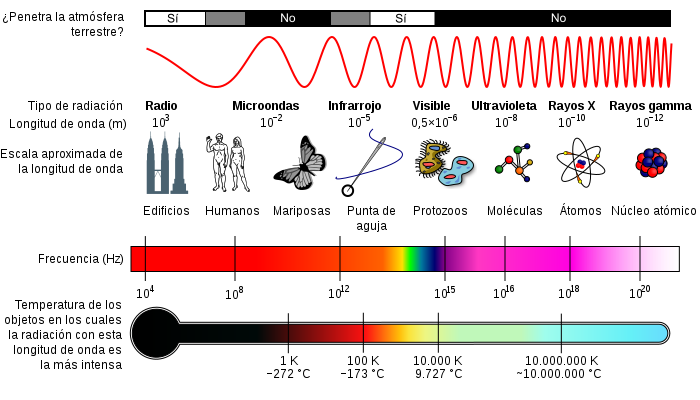
\includegraphics[width=0.75\textwidth]{images/espectro.png}
\caption{Espectro Electromagnético adaptada por~\cite{wikies} de~\cite{NASAEspectro} en la que se muestra la longitud de onda de cada agrupación}

\end{figure}
\section{Resolución} 
La resolución de una imagen indica la cantidad de detalles que puede observarse en esta. Tener mayor resolución se traduce en obtener una imagen con más detalle o calidad visual. Según~\cite{Wulder1998} la resolución es la medida de variación de un sensor para conseguir un valor.
\begin{itemize}
 \item \textbf{Resolución Espacial}\newline
Es la cantidad de información que representa un pixel~\cite{Wulder1998}, siendo el caso que un objeto puede estar representado por un solo pixel de 100 metros cuadrados o por 100 pixeles de 1 metro cuadrado. 
\begin{figure}[H]
    \centering
    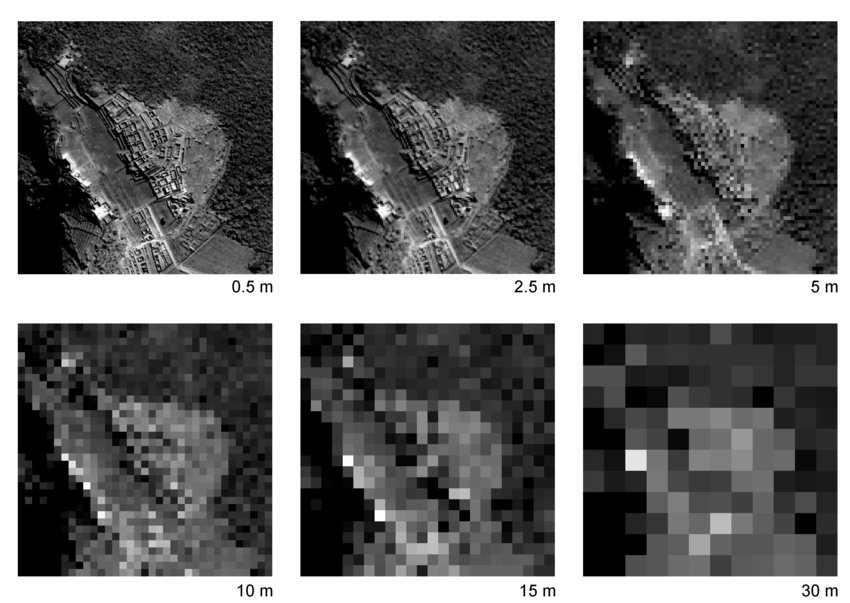
\includegraphics[width = 0.8\textwidth]{images/02theory/espacial.png}
    \caption{Distintas resoluciones espaciales para la misma zona}
    \label{fig:resolucionEspacial}
\end{figure}

Como se aprecia en la \figurename~\ref{fig:resolucionEspacial} cuando se tiene una mayor resolución espacial los objetos tienen un mayor grado de detalle.


\item \textbf{Resolución Espectral}\newline
 Hace referencia a la cantidad del espectro electromagnético se esta midiendo y en cuantos canales se separa, es decir que si la imagen fue tomada en un amplio espectro y el tamaño de los canales es corto tendrá una mejor resolución espectral~\cite{wulder2012remote}.
 \begin{figure}[H]
     \centering
     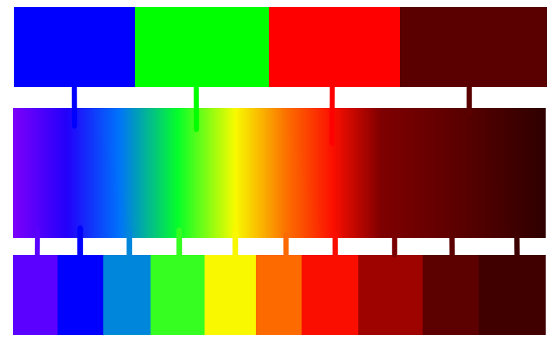
\includegraphics[width=0.6\textwidth]{images/02theory/resolucionespectralCortada.png}
     \caption[Resolución espectral]{Se muestra que en determinado rango del espectro electromagnético se puede usar divisiones más pequeñas para obtener más canales espectrales o mejor resolución espectral}
     \label{fig:resolucionEspectral}
 \end{figure}
 
 
\item \textbf{Resolución Temporal}\newline
 Se toma en cuenta que la resolución temporal es la frecuencia por la que un satélite puede tomar información de una zona~\cite{Wulder1998}.
\begin{figure}[H]
    \centering
    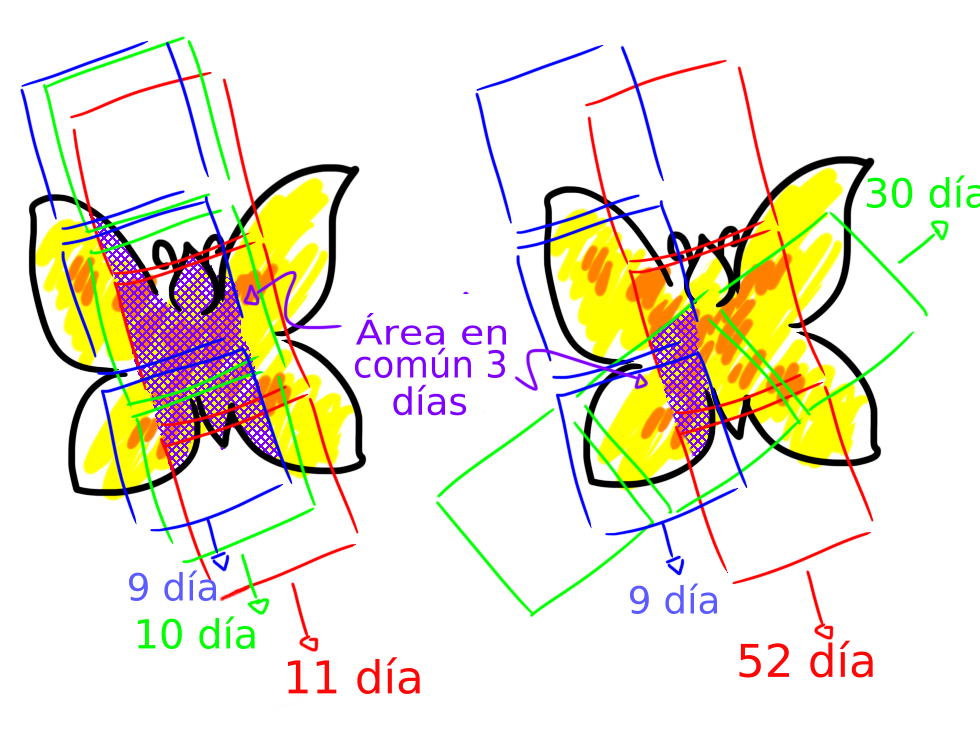
\includegraphics[width=0.5\textwidth]{images/02theory/resolucionTemporalEspa.png}
    \caption[Resolución Radiométrica]{Resolución Temporal: Como se muestra en la figura la mejora de la resolución temporal facilitara la obtención de información multitemporal de una zona}
    \label{fig:my_label}
\end{figure} 
 
\item \textbf{Resolución Radiométrica}\newline
Se refiere a la cantidad de bits usados para representar la información, esto determinará que tan selectivo es el sensor~\cite{wulder2012remote}. 
\begin{figure}[H]
    \centering
    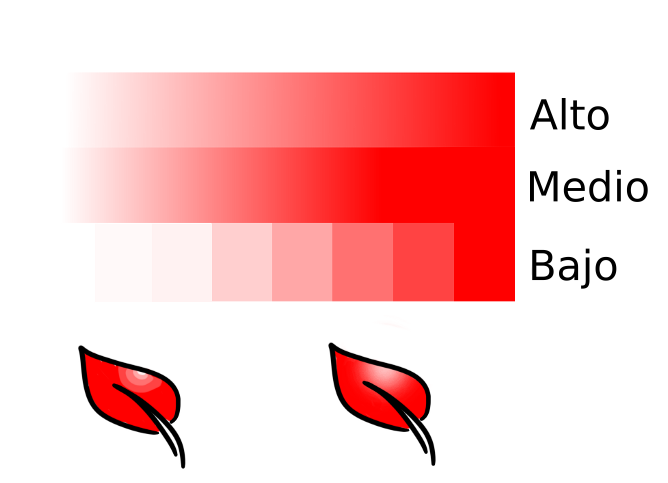
\includegraphics[width=0.6\textwidth]{images/02theory/resolucionRadiometrica.png}
    \caption[Resolución Radiométrica]{Resolución Radiométrica: Como se muestra en la hoja izquierda mientras menor sea la resolución radiométrica menos tonalidades tendremos de un valor}
    \label{fig:my_label}
\end{figure}
\end{itemize}

\section{Teledetección }
La Teledetección es una técnica por medio de la cual se obtiene información útil de un objeto, área o fenómeno, a través del análisis e interpretación de datos adquiridos por un equipo que no está en contacto físico con el objeto, área o fenómeno bajo investigación~\cite{jensen1987introductory}. 


La Teledetección espacial es una técnica que permite adquirir información de la superficie terrestre o marina y la atmósfera desde sensores instalados en plataformas espaciales, por ser una técnica que no esta en contacto directo con el objeto requiere que entre el sensor y el objeto haya un flujo de información.
\subsection{Usos}
Según el Servicio Geológico de los Estados Unidos algunos usos de la teledetección son~\cite{USGS}:
\begin{itemize}
 \item Las cámaras en satélites y aviones toman imágenes de grandes áreas en la superficie de la Tierra, lo que nos permite ver mucho más de lo que podemos desde una vista desde el suelo.
 \item Los sistemas de sonar en los barcos se pueden usar para crear imágenes del fondo del océano sin necesidad de viajar al fondo del océano.
  \item Se pueden usar cámaras en satélites para hacer imágenes de los cambios de temperatura en los océanos.
\end{itemize}
Algunos usos específicos de las imágenes satelitales de la tierra son: 
\begin{itemize}

 \item Los incendios forestales grandes pueden ser mapeados desde el espacio, permitiendo a los guardabosques ver un área mucho mayor que desde el suelo.
 \item Rastrear nubes para ayudar a predecir el clima u observar volcanes en erupción, y ayudar a observar tormentas de polvo.
 \item Rastrear el crecimiento de una ciudad y los cambios en tierras de cultivo o bosques durante varios años o incluso décadas.
.
\end{itemize}
\subsection{Satélites de observación}
Los satélites de observación son satélites artificiales, su principal función de estos es la obtención de información mediante sensores, que pueden ser clasificados de 2 formas~\cite{campbell2011introduction}: 
\begin{itemize}
 \item \textbf{Activos} Generan su propia fuente de medición, ejemplo: 
 \begin{itemize}
  \item \textbf{SAR}\newline El SAR (Synthetic Aperture Radar en español radar de apertura sintética) es un radar activo que emite la energía en el intervalo de frecuencias de microondas en un período pequeño de tiempo y recibe los ecos provenientes de reflexiones de la señal en los objetos dando lugar a una apertura sintética~\cite{brown1967synthetic}. 
  \item \textbf{Lidar}\newline Un lídar (un acrónimo del inglés Light Detection and Ranging o Laser Imaging Detection and Ranging) es un dispositivo que permite determinar la distancia desde un emisor láser a un objeto o superficie. La distancia al objeto se determina midiendo el tiempo de retraso entre la emisión del pulso y su detección a través de la señal reflejada~\cite{Lim2003}.
  
 \end{itemize}
 \item \textbf{Pasivos} Estos obtienen información midiendo energía externa, ejemplo: \begin{itemize}
  \item \textbf{Satélites Ópticos}\newline En este caso la energía creado por el sol reflejada de la tierra es medida usando sensores, luego la información recobrada es usada para la construcción de una nueva imagen~\cite{elachi2006introduction}. La información obtenida usualmente esta fuera del rango del espectro electromagnético visto por el hombre.
 \end{itemize}
 
\end{itemize}
 
\subsection{Imágenes satelitales}
Una imagen satelital o imagen de satélite es la representación de la información capturada por un satélite~\cite{leon2002introduccion}.

\extrarowheight = -0.5ex
\renewcommand{\arraystretch}{2.25}
 \begin{table}[H]
\centering

\caption{Tabla de satélites adaptado de~\cite{unsalan2013multispectral}}
\resizebox{16cm}{!}{% <------ Don't forget this %
\begin{tabular}{|M{0.14\textwidth}|M{0.16\textwidth}|
   M{0.15\textwidth}|M{0.15\textwidth}|
   M{0.14\textwidth}|M{0.25\textwidth}|}
   \hline
 \cellcolor[HTML]{dcdcdc}\color[HTML]{000000} \textbf{Sensor} &
 \cellcolor[HTML]{dcdcdc}\color[HTML]{000000} \textbf{Resolución Espacial} Pancromática ($\SI{}{\metre}$) &
 
\cellcolor[HTML]{dcdcdc}\color[HTML]{000000} \textbf{Resolución Espacial Multiespectral ($\SI{}{\metre}$)} &

\cellcolor[HTML]{dcdcdc}\color[HTML]{000000} \textbf{Resolución Espectral ($ \SI{}{\micro\metre}$)} & 
\cellcolor[HTML]{dcdcdc}\color[HTML]{000000} \textbf{Resolución Temporal (días) } & \cellcolor[HTML]{dcdcdc}\color[HTML]{000000} \textbf{Bandas }  \\
 \hline
 

Landsat & 15 &  30  & 0.45 a 2.35               &  16          & BGR, NIR, SWIR1, SWIR2, TIR, PAN           \\  
SPOT        & 2.5 &10         & 0.50 a 1.75        & 5   & BGR, NIR, PAN        \\  

IRS       & 5 &23.5        & 0.50 a 1.70        & 5 & BGR, NIR, PAN         \\  
 
IKONOS        & 1 & 4        & 0.45 a 0.85        &  3 & BGR, NIR, PAN           \\  
QuickBird       & 0.61 &2.44         & 0.45 a 0.90        & 3   & BGR, NIR, PAN          \\  

FormoSat        & 2  &8         & 0.45 a 0.90        & 1 &BGR, NIR, PAN          \\  

CartoSat        & 2.5& N/A        & N/A        & 5  & PAN      \\  

WorldView       & 0.46 & 1.8         & 0.40 a 1.04        & 1.1   & BGR, NIR, SWIR1, SWIR2, TIR, PAN         \\  
ALOS       & 2.5 & 10         & 0.42 a 0.89        & 2  & BGR, NIR, PAN         \\  

GeoEye        & 0.41  &1.65        & 0.45 a 0.90        & 3   &BGR, NIR, PAN           \\  
Airborne        & 1 a 25 & 1 a 25         & 0.42 a 14.00        & N/A    & 1 a 224       \\  
Sentinel        & 10 & 20 o 60         & 0.443 a 2.190        & 10   & BGR, NIR, SWIR1, SWIR2, TIR, PAN        \\  
PeruSat       & 0.7 & 2.8 & 0.45 a 0.89        & 0.5  & BGR, NIR, PAN     
\\\hline
\end{tabular}% <------ Don't forget this %
}

\label{tab}%
\end{table}%

\section{Inteligencia Artificial}
En el \tablename  ~\ref{cuadroIA} adaptado de~\cite{russell2004inteligencia} se muestran algunas definiciones de inteligencia artificial. Las que aparecen en la parte superior se refieren a procesos mentales y al razonamiento, mientras que las de la parte inferior aluden a la conducta. Las definiciones de la izquierda miden el éxito en términos de la fidelidad en la forma de actuar de los humanos, mientras que las de la derecha toman como referencia un concepto ideal de inteligencia, que llamaremos racionalidad. Un sistema es racional si hace lo correcto, en función de su conocimiento.


 \begin{table}[H]
\centering

\caption{Cuadro de definiciones de Inteligencia Artificial adaptado de~\cite{russell2004inteligencia}}
\label{cuadroIA}
\begin{tabular}{|M{0.45\textwidth}|M{0.45\textwidth}|}
   \hline
 \cellcolor[HTML]{dcdcdc}\color[HTML]{000000} \textbf{Sistemas que piensan como humanos} &
 \cellcolor[HTML]{dcdcdc}\color[HTML]{000000} \textbf{Sistemas que piensan racionalmente}
 
 \\ \hline
 \begin{itemize}
  \item El nuevo y excitante esfuerzo de hacer que los computadores piensen... máquinas con mentes, en el más amplio sentido literal~\cite{Haugeland1985}.
\item La automatización de] actividades que vinculamos con procesos de pensamiento humano, actividades como la toma de decisiones, resolución de problemas, aprendizaje...~\cite{bellman1978introduction}
 
 \end{itemize}
 

&
\begin{itemize}
 \item El estudio de las facultades mentales mediante el uso de modelos computacionales~\cite{charniak1985introduction}.
 \item El estudio de los cálculos que hacen posible percibir, razonar y actuar~\cite{winston1992learning}.
 
\end{itemize}
 \\ \hline
 \cellcolor[HTML]{dcdcdc}\color[HTML]{000000} \textbf{Sistemas que actúan como humanos
} 
&
 \cellcolor[HTML]{dcdcdc}\color[HTML]{000000} \textbf{Sistemas que actúan racionalmente}
 \\ \hline
 \begin{itemize}
  \item El arte de desarrollar máquinas con capacidad para realizar funciones que cuando son realizadas por personas requieren de inteligencia~\cite{kurzweil1990age}.
 \item El estudio de cómo lograr que los computadores realicen tareas que, por el momento, los humanos hacen mejor~\cite{rich1991artificial}.
 
 \end{itemize}
&
\begin{itemize}
 \item La Inteligencia Computacional es el estudio del diseño de agentes inteligentes.~\cite{poole1998computational}
 \item IA... está relacionada con conductas inteligentes en artefactos~\cite{nilsson1998artificial}.
\end{itemize}

 \\ 
\hline
\end{tabular}%

\label{tab:addlabel}%
\end{table}%
\subsection{Visión computacional}
La principal función de la visión es reconocer y localizar objetos en el ambiente mediante el procesamiento de las imágenes. La visión computacional es el estudio de estos procesos, para entenderlos y construir maquinas con capacidades similares~\cite{sucar2011vision}.
Algunas definiciones de visión son:
\begin{itemize}
  \item Visión es saber que hay y donde mediante la vista (Aristóteles).
  \item Visión es recuperar de la información de los sentidos (vista) propiedades validas del mundo exterior, Gibson~\cite{gibson2014ecological}.
  \item  Visión es un proceso que produce a partir de las imágenes del mundo exterior una descripción que es útil para el observador y que no tiene información irrelevante, Marr~\cite{marr1982vision}.
\end{itemize}
\subsection{Aprendizaje profundo}
Las RNA (redes neuronales artificiales) son modelos predictivos basados en la estructura biológica del cerebro humano. Una RNA se construye mediante la vinculación de entrada nodos con conexiones ponderadas a los nodos de salida a través de uno o más
capas de nodos ocultos~\cite{rumelhart1986learning}.


El aprendizaje profundo es un enfoque caracterizado por tener múltiples niveles que sirven para abstraer información de un conjunto de datos~\cite{lecun2015deep}. Una de las estructuras más utilizadas son las redes neuronales convolucionales.


En una red neuronal normal las entradas están desplegadas de manera lineal, es decir las redes son operadas linealmente hacia la siguiente capa. En el caso de una red neuronal convolucional las capas tienen más de una dimensión a esto se le conoce como capas convolucionales, esto provee información espacial que puede ser utilizada por la red neuronal para una mejor extracción de características. La forma en la cual se pasa información de una capa otra es mediante convoluciones que es la transformación de un valor a otro

\section{Redes Neuronales}
\subsection{Redes Neuronales Convencionales}
\label{section:marcoTeorico:redesneuronales}
Para~\cite{Haykin1994} una red neuronal o unidad de procesamiento es una máquina diseñada para modelar la forma en la que el cerebro realiza una actividad, la define además como un procesador distribuido masivamente paralelo formado por unidades de procesamiento simples (neuronas) que son propensos a almacenar conocimiento y ponerlo a disposición para su uso. Cada neurona recibe una serie de entradas a través de interconexiones y emite una salida. Se identifican 3 elementos básicos del modelo como sigue:
\begin{itemize}
\item Conjunto de sinapsis o enlaces de conexión que reemplazan a las conexiones sinápticas del cerebro humano, caracterizadas por tener un peso equivalente a la efectividad de la sinapsis, en específico con respecto al peso de una neurona en la~\figurename~\ref{figure:RedNeuronal}, en $w_{kj}$ el primer subíndice representa a la neurona propia, el segundo subíndice se refiere a la señal de entrada, formando así el peso neuronal.
\item Una función de propagación o de red, consiste en la sumatoria de cada entrada multiplicada por el peso de su interconexión (valor neto). Si el peso es positivo, la conexión se denomina excitatoria; si es negativo, se denomina inhibitoria, las operaciones describen una combinación lineal.
\item Una función activación, que se aplica al valor devuelto por la función de propagación. Se utiliza para acotar la salida de la neurona y viene dada por la interpretación que se da a las salidas. Algunas de las más utilizadas son la función sigmoidea (para obtener valores en el intervalo [0, 1] y la tangente hiperbólica (para obtener valores en el intervalo [-1, 1]).
\end{itemize}

\begin{figure}[H]
  \centering
    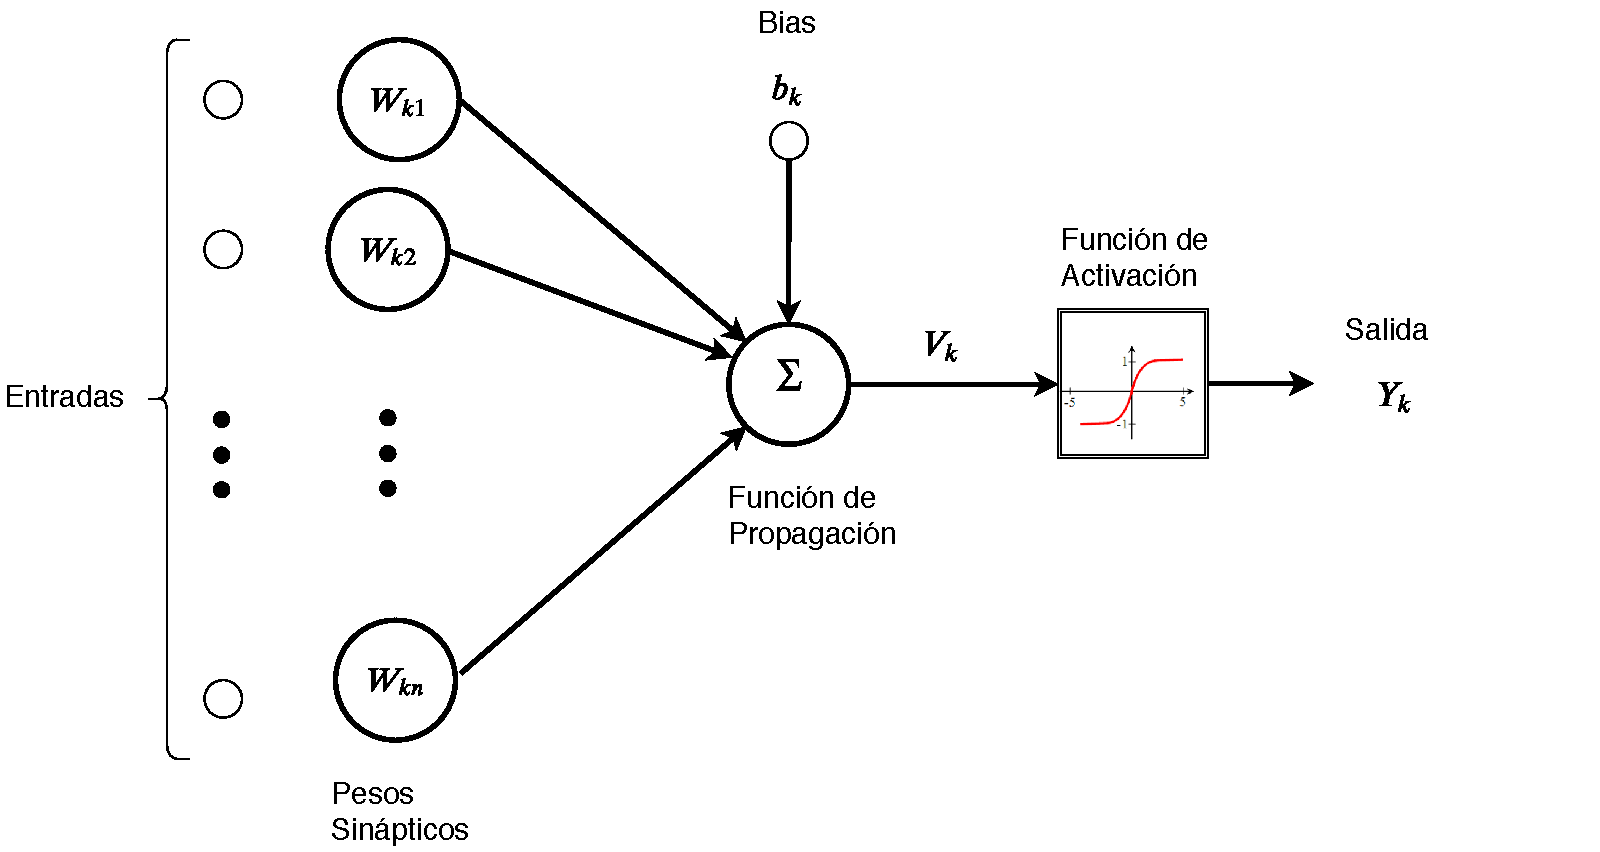
\includegraphics[width=0.9\textwidth]{images/redNeuronal.pdf}
  \caption[Arquitectura general Red Neuronal]{Modelo arquitectónico de una Red Neuronal adaptado de~\cite{Haykin1994}.}
  \label{figure:RedNeuronal}
\end{figure}

El modelo de red neuronal en la \figurename~\ref{figure:RedNeuronal} incluye un bias $b_{k}$, se puede describir la neurona $k$ con las siguientes ecuaciones:
\begin{equation}
  u_{k} = \sum_{j=1}^{n}x_{i} = w_{kj} \cdot x_{j}   
\end{equation}

\begin{equation}
  y_{k} =\varphi (u_{k}+b_{k})  
\end{equation}
\begin{equation}
  v_{k} = u_{k}+b_{k}  
\end{equation}

\subsection{Redes Neuronales Convolucionales}
 Una Red Neuronal Convolucional o \gls{CNN} por sus siglas en ingles (Convolutional Neural Network) es una red neuronal especial debido que procesa la data de manera topológica. Las \gls{CNN} han tenido tremendo éxito en aplicaciones prácticas, el nombre red convolucional  indica que la red emplea una operación matemática llamada convolución. La red neuronal convolucional es una red neuronal común que usa convoluciones en lugar de multiplicaciones matriciales en al menos alguna de sus capas.
\subsection{Función de perdida}
En el contexto de un algoritmo de optimización, la función utilizada para evaluar una solución candidata (es decir, un conjunto de ponderaciones) se conoce como la función objetivo.

Podemos buscar maximizar o minimizar la función objetivo, lo que significa que estamos buscando una solución candidata que tenga la puntuación más alta o más baja, respectivamente.

Normalmente, con las redes neuronales, buscamos minimizar el error. Como tal, la función objetivo a menudo se denomina función de costo o función de pérdida y el valor calculado por la función de pérdida se denomina simplemente "pérdida".
\subsection{Operaciones en redes Neuronales Convolucionales}
\subsubsection{Convolución }
\label{subsec:convolucion}

En el trabajo de \cite{Dumoulin2016} se mecían que la principal operación en las redes neuronales clásicas es la transformación afín: un vector se recibe como entrada y se multiplica con una matriz para producir una salida (a la que generalmente se agrega un vector de polarización antes de pasar el resultado a través de una no linealidad). Esto es aplicable a cualquier tipo de entrada, ya sea una imagen, un clip de sonido o una colección desordenada de características: sea cual sea su dimensionalidad, su representación siempre puede ser aplanada en un vector antes de la transformación. No obstante imágenes, clips de sonido y muchos otros tipos similares tienen una estructura intrínseca. Más formalmente, comparten estas importantes propiedades:
\begin{itemize}
    \item  Se almacenan como matrices multidimensionales.
\item Cuentan con uno o más ejes para los que es importante el ordenamiento (por ejemplo, ejes de ancho y alto para una imagen, eje de tiempo para un clip de sonido).
\item Un eje, llamado el eje del canal, se usa para acceder a diferentes vistas de los datos (por ejemplo, los canales rojo, verde y azul de una imagen en color, o los canales izquierdo y derecho de una pista de audio estéreo).
\end{itemize}

Estas propiedades no se explotan cuando se aplica una transformación afín, de hecho, todos los ejes se tratan de la misma manera y la información topológica no se tiene en cuenta. Sin embargo, aprovechar la estructura implícita de los datos puede resultar muy útil para resolver algunas tareas, como la visión artificial y el reconocimiento de voz, y en estos casos sería mejor preservarlo. Aquí es donde entran en juego las convoluciones discretas.Una convolución discreta es una transformación lineal que preserva esta noción de orden. Es esparcido (solo unas pocas unidades de entrada contribuyen a una unidad de salida determinada) y reutiliza los parámetros (los mismos pesos se aplican a múltiples ubicaciones en la entrada)
La \figurename~\ref{fig:convolucionArimetica} provee un ejemplo de lo que una convolución discreta. La grilla azul claro es llamada \gls{Feature Map} de entrada, pero es bastante común tener varios mapas de características amontonados uno sobre otro. Un \gls{kernel}(cuadrado plomo) pasa atreves del \gls{Feature Map} de entrada. En cada posición, se obtiene el producto entre cada uno de los elementos del \gls{kernel} y la entrada que se sobrelapan, el resultado final es obtenido sumando los resultados de los productos. Este proceso puede ser repetido con distintos \gls{kernel}s para formar diferentes \gls{Feature Map}s de salida. En caso de que se presenten varios \gls{Feature Map}s de entrada el \gls{kernel} tendrá que ser tridimensional (o equivalente a un \gls{kernel} por cada mapa de características de entrada).


%1 A kernel (shaded area) of value 
%slides across the input feature map. At each location, the product between
%each element of the kernel and the input element it overlaps is computed and
%the results are summed up to obtain the output in the current location. The
%procedure can be repeated using different kernels to form as many output feature
%maps as desired (Figure 1.3). The final outputs of this procedure are called
%output feature maps. 2 If there are multiple input feature maps, the kernel will
%have to be 3-dimensional – or, equivalently each one of the feature maps will
%be convolved with a distinct kernel – and the resulting feature maps will be
%summed up elementwise to produce the output feature map.
%The convolution depicted in Figure 1.1 is an instance of a 2-D convolution,
%but it can be generalized to N-D convolutions. For instance, in a 3-D convolu-
%tion, the kernel would be a cuboid and would slide across the height, width and
%depth of the input feature map.
%The collection of kernels defining a discrete convolution has a shape corre-
%sponding to some permutation of (n, m, k 1 , . . . , k N ), where
%n ≡ number of output feature maps,
%m ≡ number of input feature maps,
%k j ≡ kernel size along axis j.
%The following properties affect the output size o j of a convolutional \gls{Layer}
%along axis j:
%• i j : input size along axis j,
%• k j : kernel size along axis j,
%• s j : stride (distance between two consecutive positions of the kernel) along
%axis j,
%• p j : zero padding (number of zeros concatenated at the beginning and at
%the end of an axis) along axis j.
%For instance, Figure 1.2 shows a 3 × 3 kernel applied to a 5 × 5 input padded
%with a 1 × 1 border of zeros using 2 × 2 strides.
%Note that strides constitute a form of subsampling. As an alternative to
%being interpreted as a measure of how much the kernel is translated, strides can
%also be viewed as how much of the output is retained. For instance, moving
%the kernel by hops of two is equivalent to moving the kernel by hops of one but
%retaining only odd output elements (Figure 1.4).

\begin{figure}[H]
    \centering
    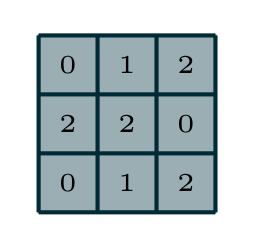
\includegraphics[width=0.2\textwidth]{images/convolucion/featuremap.png}
    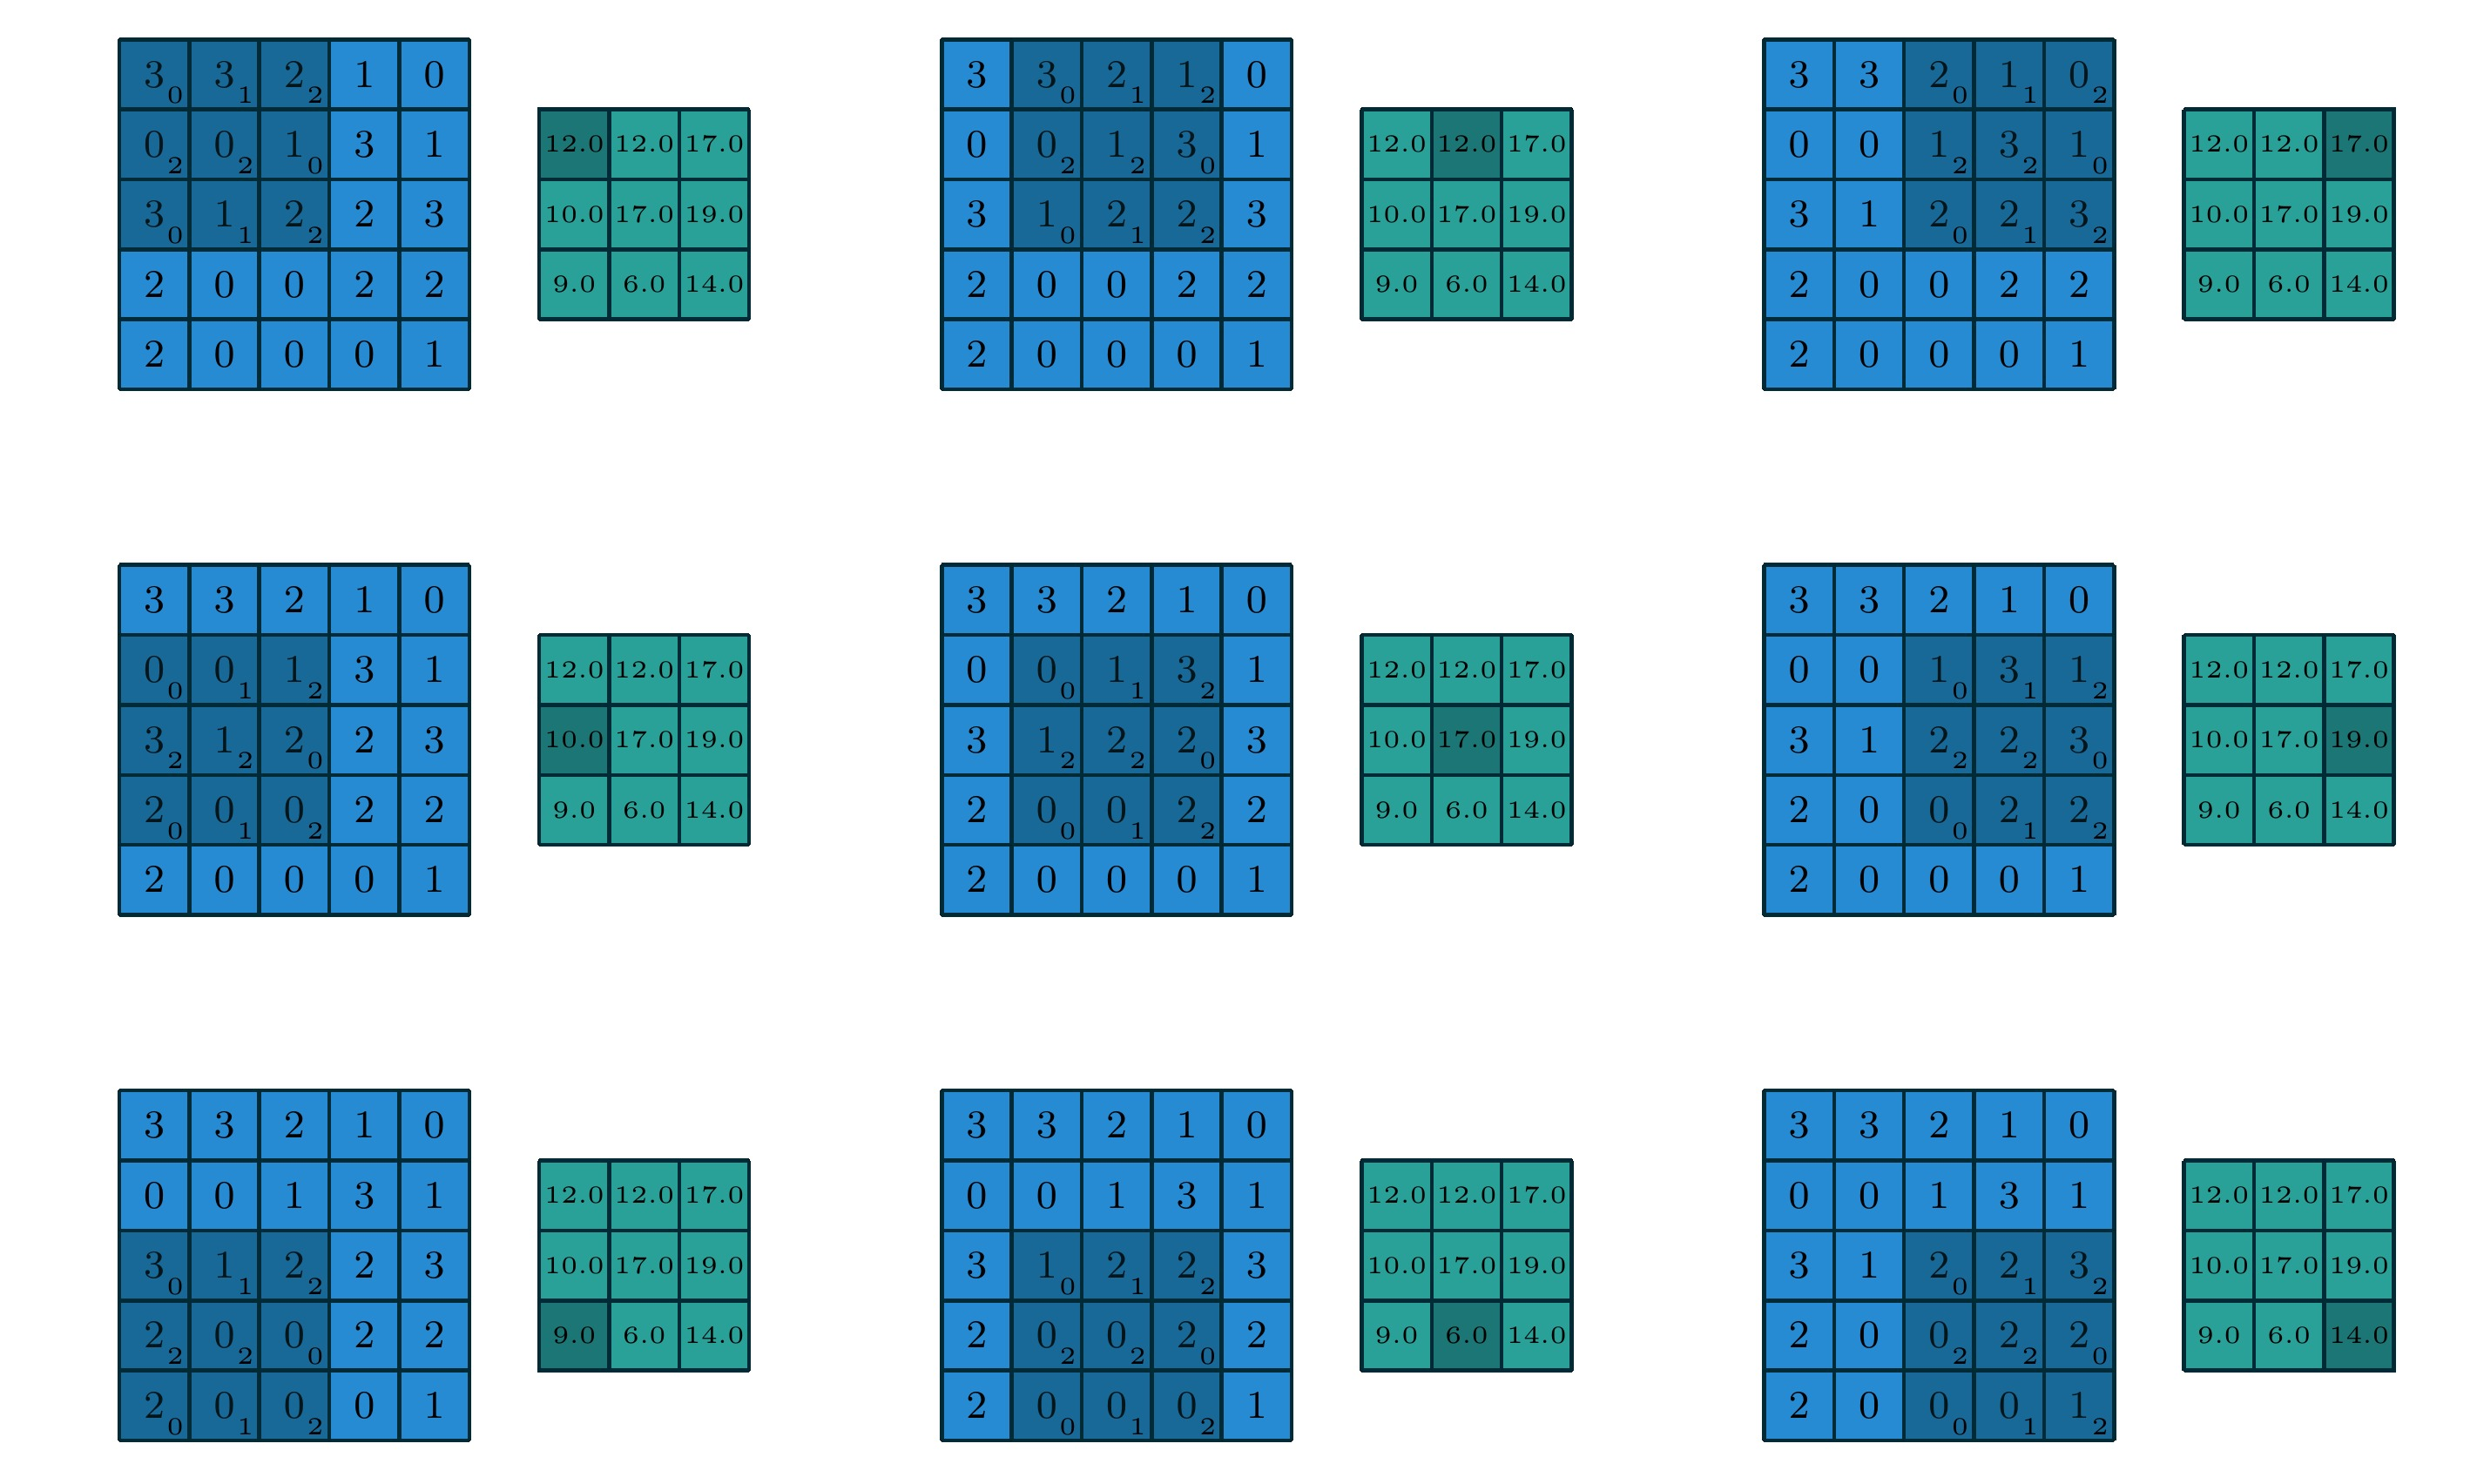
\includegraphics[width=1\textwidth]{images/convolucion/ima11.jpg}
    \caption{Muestra de la convolución aritmética en 2 dimensiones}
    \label{fig:convolucionArimetica}
\end{figure}

        
        En el caso practico más sencillo, el valor de la salida de esta operación con una entrada de dimensiones ($N, C_{in}, H, W$) y de una salida de dimensiones ($N, C_{out}, H_{out}, W_{out}$)  esta descrito por la siguiente fórmula:
\begin{equation}
    out(N_i, C_{out_j})=bias(Cout_j)+\sum_{k=0}^{C_{in}-1}weight(C_{out_j},k)\star input(N_i, k)
\end{equation}

Donde $\star$ es el operador de convolución que fue descrito en la sección \ref{subsec:convolucion}, N es el tamaño de \gls{Batch}, C denota el numero de canales, H es la altura de las entradas, y W es el ancho.

Las convoluciones tienen los siguientes parámetros de configuración:
\begin{itemize}
    \item \textbf{\gls{Stride}} controla la separación entre cada paso de la convolución .
    \begin{figure}[H]
    \centering
    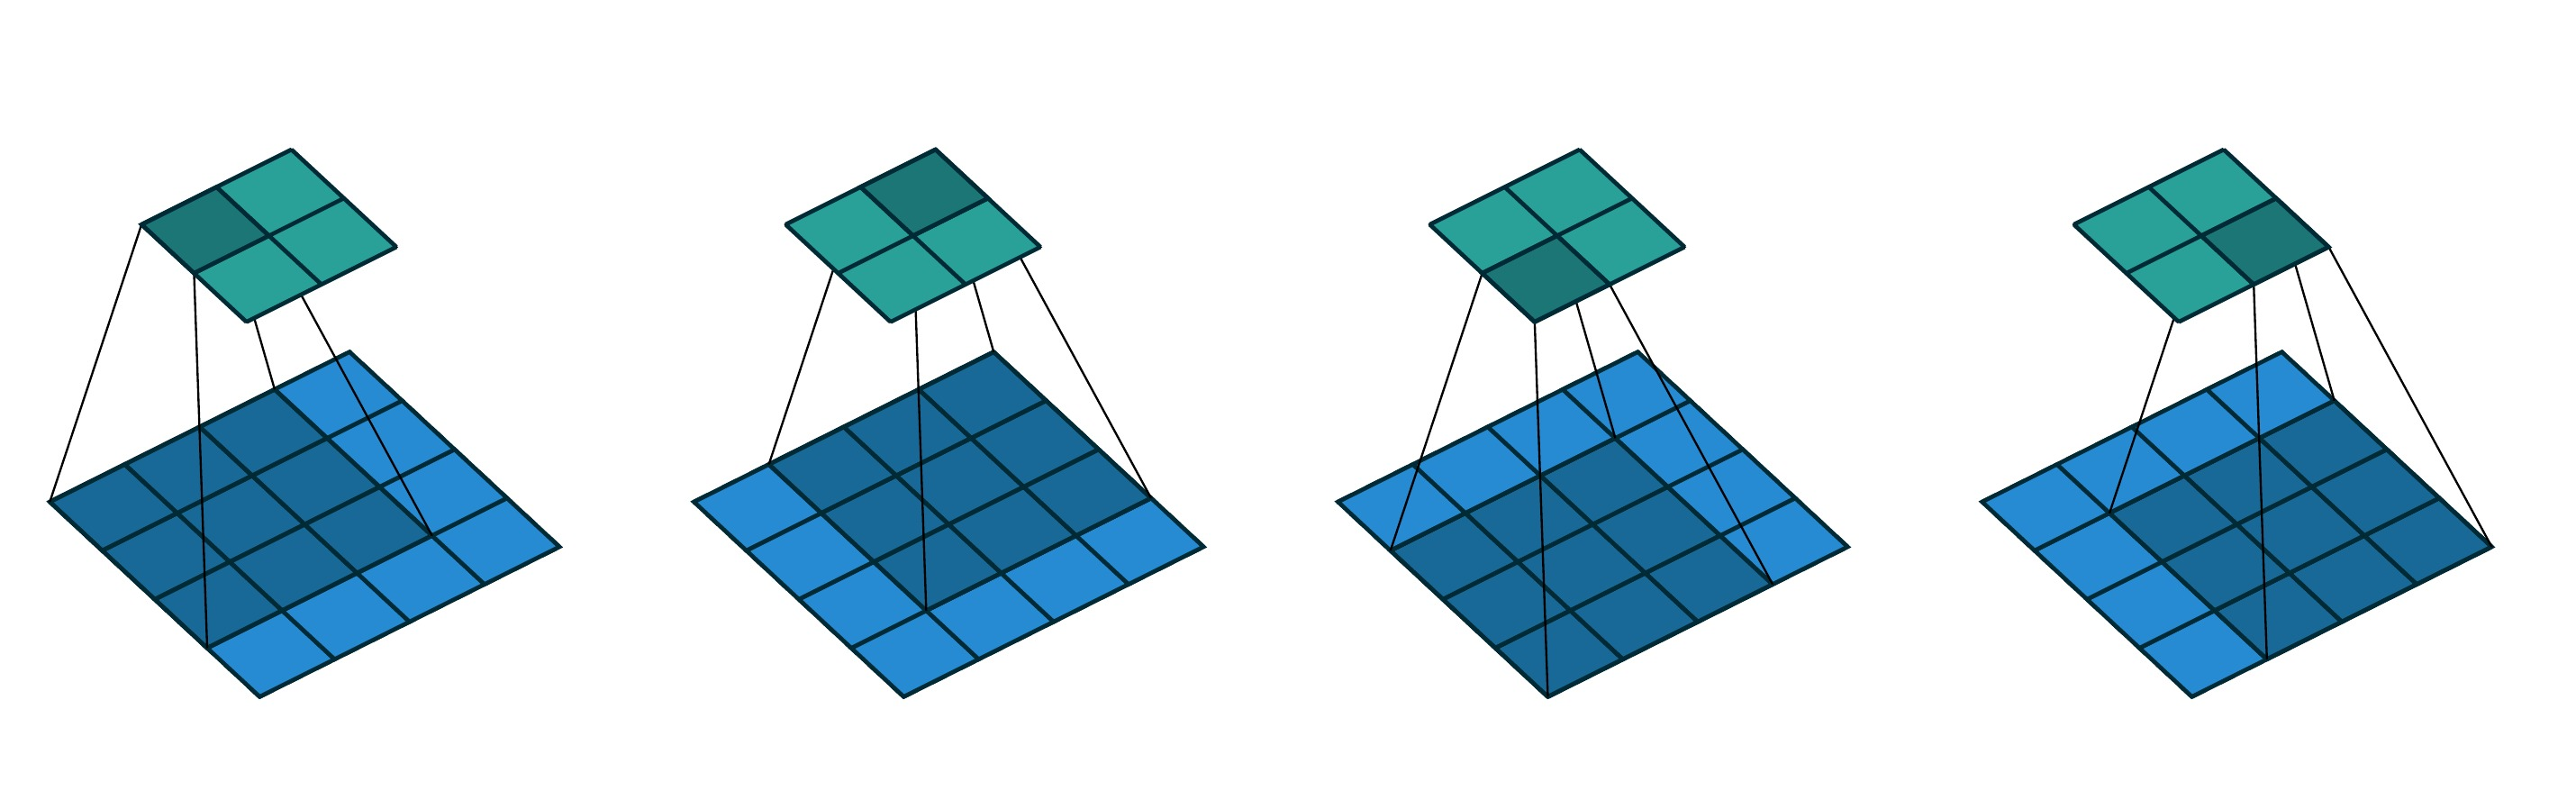
\includegraphics[width =0.9\textwidth]{images/convolucion/ima21.jpg}
    \caption{Operación de convolución con el \gls{Stride} de tamaño 1 sin padding}
    \label{fig:my_label}
\end{figure}
\begin{figure}[H]
    \centering
    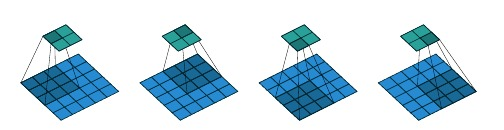
\includegraphics[width =0.9\textwidth]{images/convolucion/ima25.jpg}
    \caption{Operación de convolución con el \gls{Stride} de tamaño 2 sin padding}
    \label{fig:my_label}
\end{figure}
    \item \textbf{Padding} controla la cantidad de zeros agregados en ambos lados.
    
\begin{figure}[H]
    \centering
    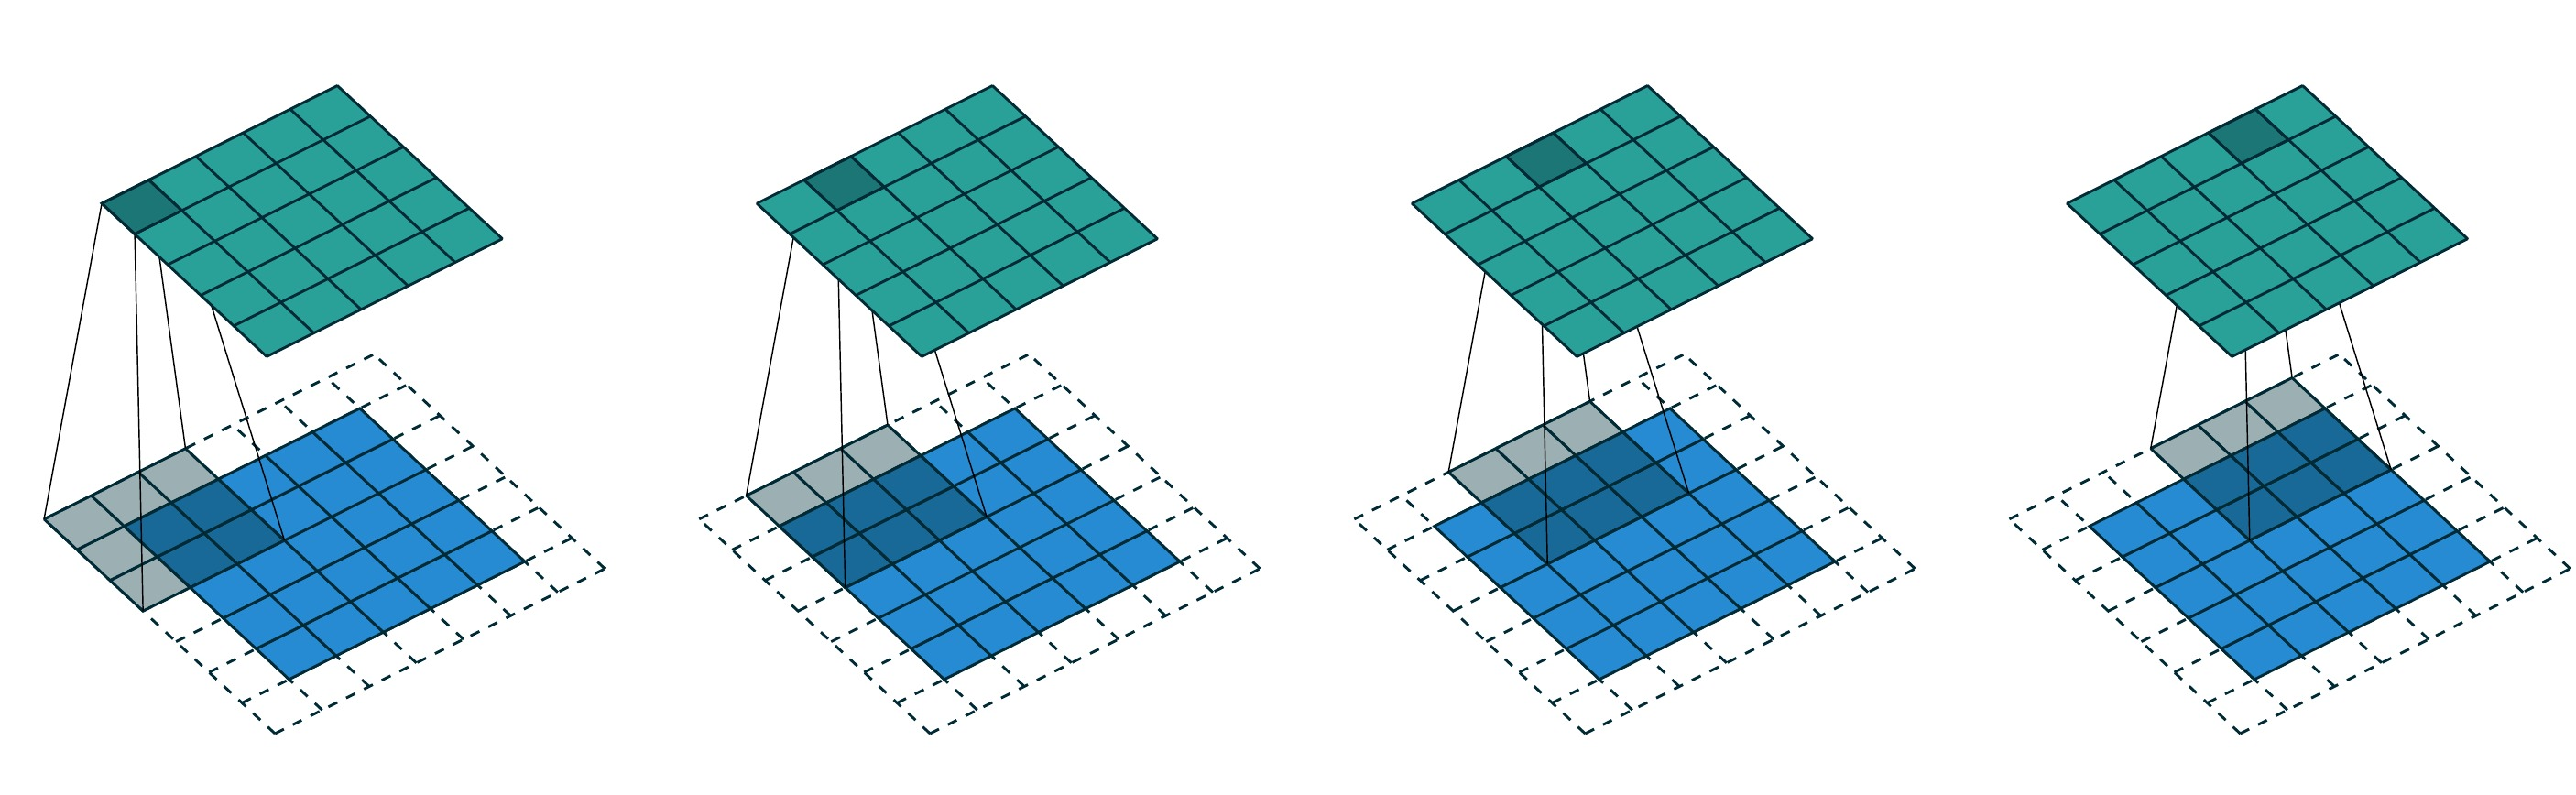
\includegraphics[width =0.9\textwidth]{images/convolucion/ima23.jpg}
    \caption{Operación de convolución con Padding de 1, \gls{Stride} de 1  }
    \label{fig:my_label}
\end{figure}
\begin{figure}[H]
    \centering
    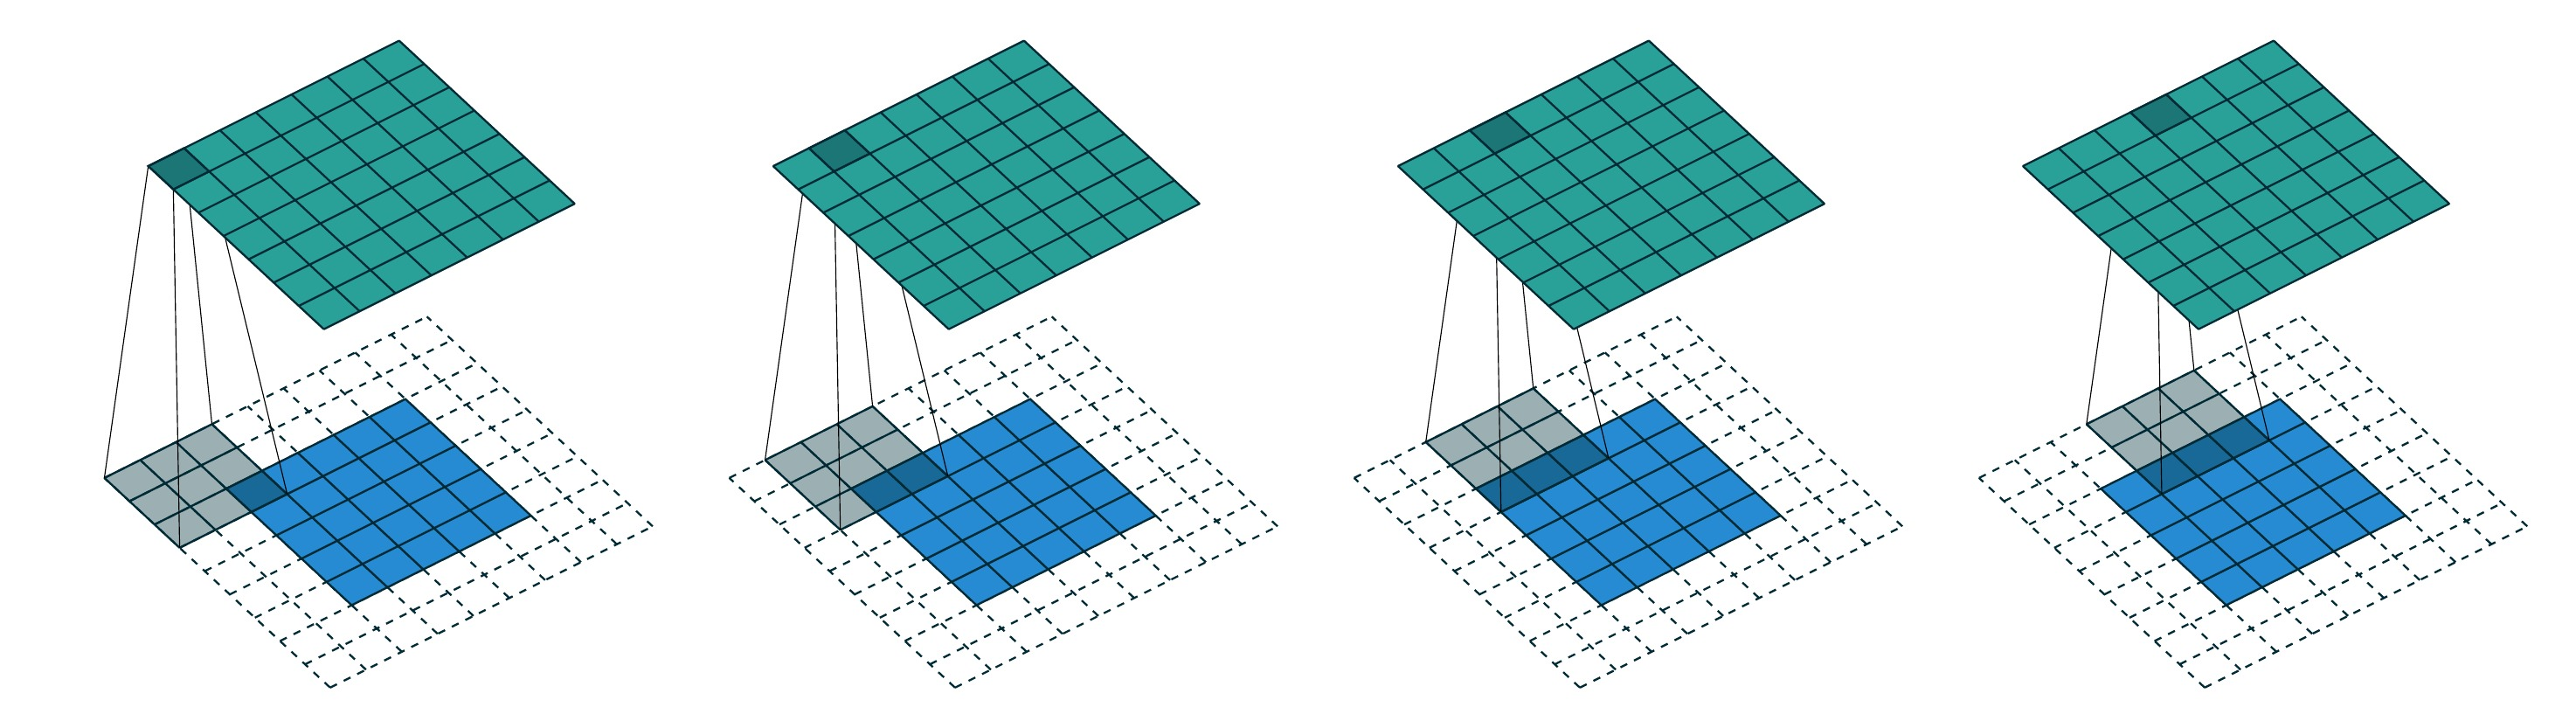
\includegraphics[width =0.9\textwidth]{images/convolucion/ima24.jpg}
    \caption{Operación de convolución con Padding de 2, \gls{Stride} de 1  }
    \label{fig:convolucionNormal}
\end{figure}

\begin{figure}[H]
    \centering
    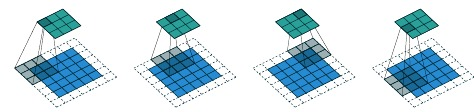
\includegraphics[width =0.9\textwidth]{images/convolucion/ima26.jpg}
    \caption{Operación de convolución con Padding de 2, \gls{Stride} de 2}
    \label{fig:my_label}
\end{figure}
    \item \textbf{Dilation} controla el espacio entre los puntos del \gls{kernel} como se ve en la \figurename~\ref{fig:dilatation}
    
\begin{figure}[H]
    \centering
    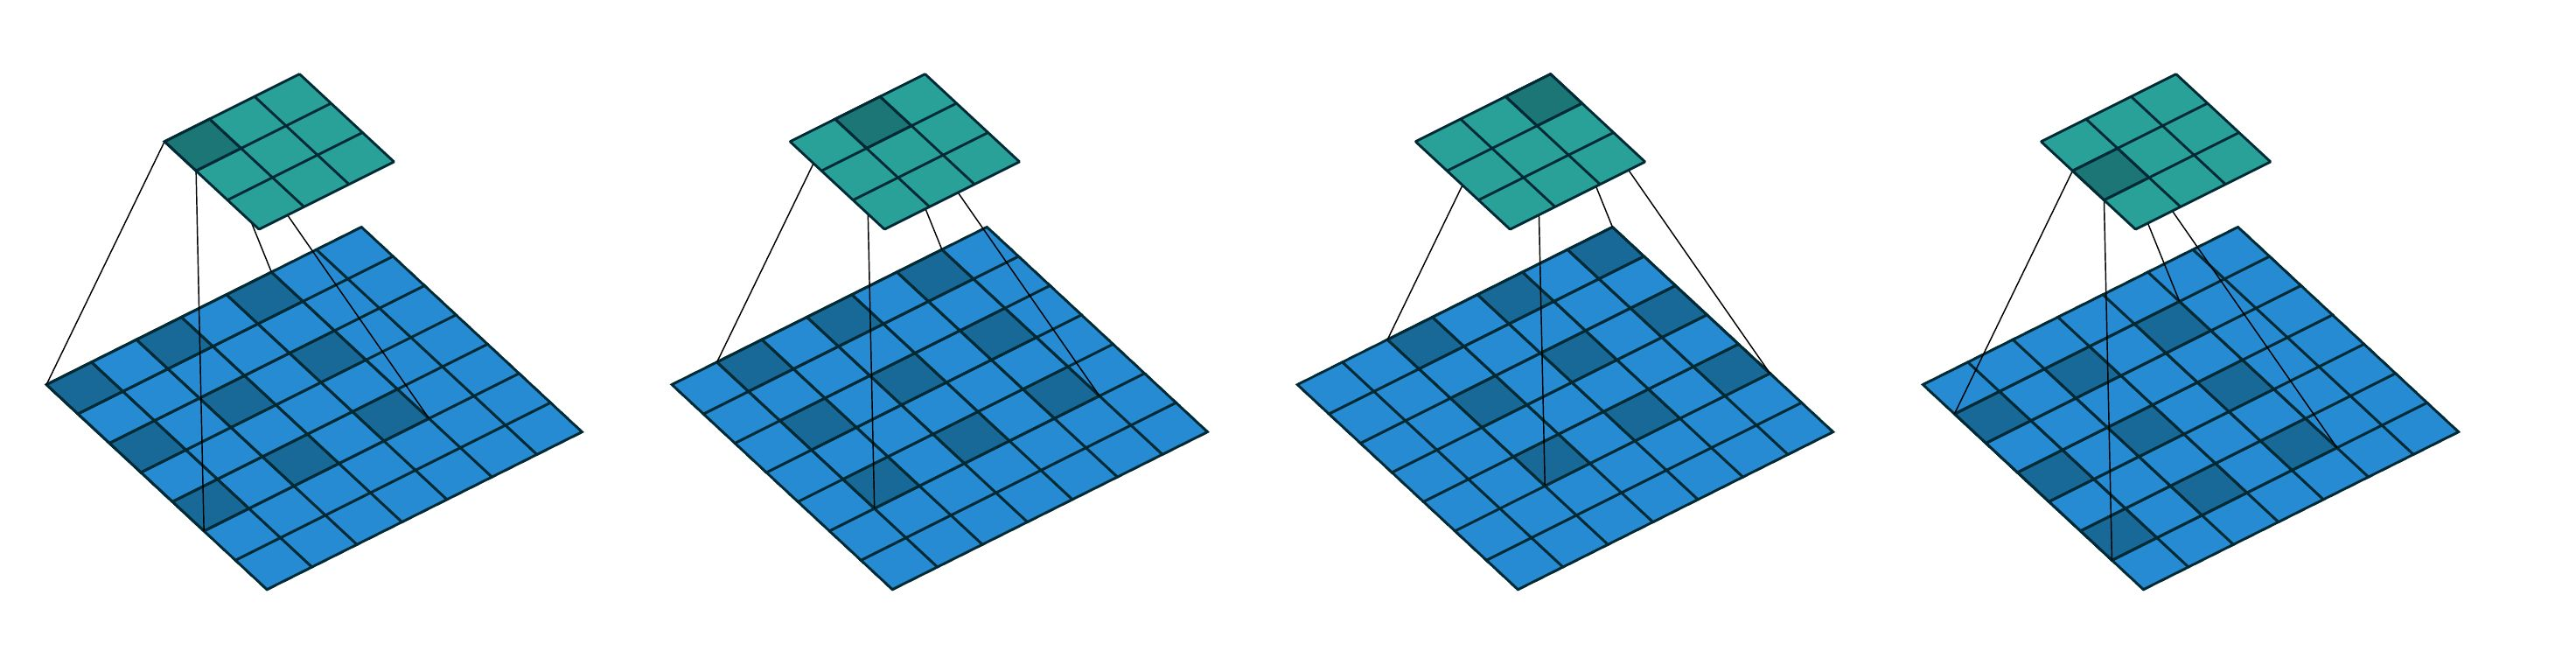
\includegraphics[width =0.9\textwidth]{images/convolucion/ima51.jpg}
    \caption{Convolución dilatada}
    \label{fig:dilatation}
\end{figure}
 
    \item \textbf{Groups} controla las conecciones entre la entrada y la salida -
            \begin{itemize}
                \item Si groups=1, todos las entradas son convolucionadas para todas las salidas.

            \item Si groups=2, la operación se convierte equivalente a tener 2 \gls{Layer}s convolucionales, cada uno ve la mitad de los canales de entrada, y produce la mitad de los canales de salida y ambos concatenados.

            \item Si groups= in\_channels, cada canal es convolucionado con su propio filtro, de tamaño: $\frac{out\_Channel}{in\_Channel}$
            \end{itemize}
            
 \begin{figure}[H]
\begin{subfigure}{.33\textwidth}
  \centering
    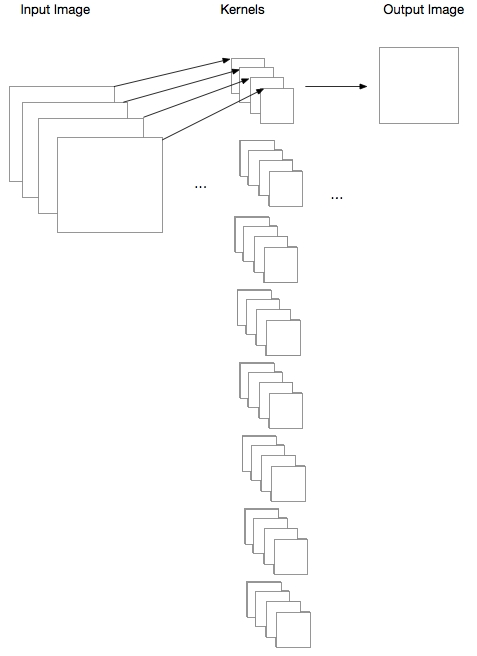
\includegraphics[width =0.9\textwidth]{images/group/g1.jpg}
  \caption{Grupo = 1}
  \label{fig:sfig1}
\end{subfigure}%
\begin{subfigure}{.33\textwidth}
  \centering
        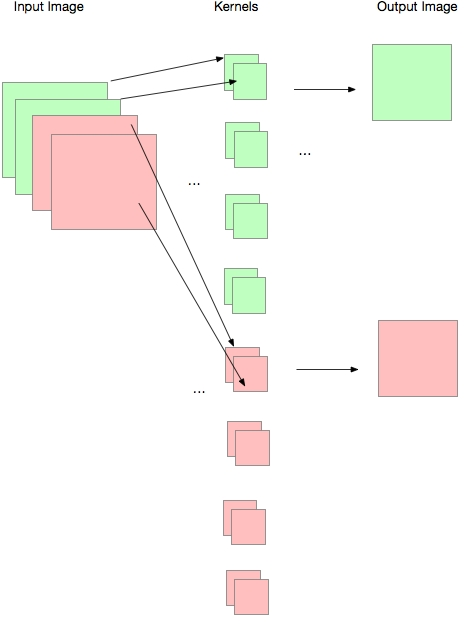
\includegraphics[width =0.9\textwidth]{images/group/g2.jpg}
  \caption{Grupo = 2}
  \label{fig:sfig2}
\end{subfigure}
\begin{subfigure}{.33\textwidth}
  \centering
    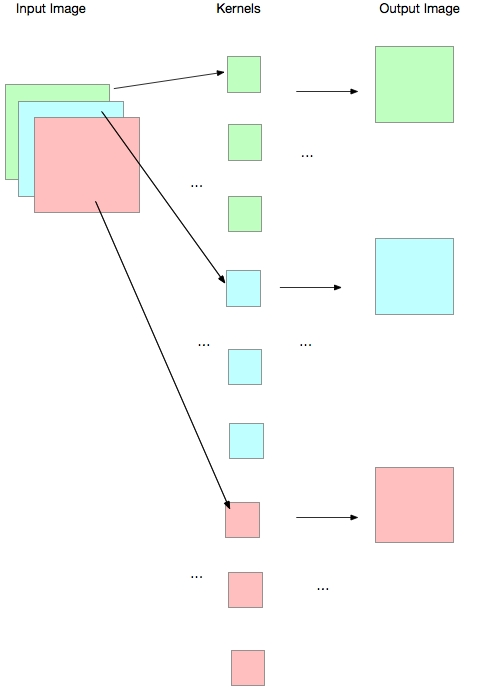
\includegraphics[width =0.9\textwidth]{images/group/g3.jpg}
  \caption{Grupo = 3}
  \label{fig:sfig2}
\end{subfigure}
\caption{Distintos tamaños de grupo}
\label{fig:convolucionGrupos}
\end{figure}
\end{itemize}
    
A continuación se pueden ver las dimensiones:
\begin{itemize}
    \item Entrada: (N, $C_{in}$, $H_{in}$, $W_{in}$)

    \item    Salida: (N, $C_{out}$, $H_{out}$, $W_{out}$) donde
       
        \begin{equation}
            H_{out}= \frac{H_{int}+2\times padding[0]-dilation[0]\times (\gls{kernel}\_ size[0]-1)-1}{\gls{Stride}[0]} 
        \end{equation}
        \begin{equation}
            W_{out}= \frac{W_{int}+2\times padding[1]-dilation[1]\times (\gls{kernel}\_ size[1]-1)-1}{\gls{Stride}[1]} 
        \end{equation}
 
\end{itemize}

\subsubsection{Pooling }
En adición a las convoluciones discretas, las operaciones de \gls{Pooling} son importante para la construcción de \gls{CNN}s. Las operaciones de \gls{Pooling} reduce el tamaño de los mapas de características usando funciones que resumen subregiones, como es el tomar el promedio o el máximo valor. 

\gls{Pooling} trabajo deslizando una ventana por la entrada y sometiendo el contenido de la ventana a una función de \gls{Pooling}. En algún sentido, el \gls{Pooling} funciona como una convolución discreta, pero reemplaza la combinación linear con otra función. La \figurename~\ref{fig:poolAverage} muestra un ejemplo de \gls{Pooling} por promedio, y la \figurename~\ref{fig:poolMax} muestra un ejemplo de \gls{Pooling} máximo.

Las siguientes propiedades afectan el tamaño de la salida $o$ de un \gls{Layer} de \gls{Pooling} 
\begin{itemize}
    \item $i$ : El tamaño de la entrada,
    \item $k$ : El tamaño de la ventana,
    \item $s$ : La distancia entre 2 ventanas consecutivas.
 
\end{itemize}
\begin{equation}
    o = \lfloor\frac{i-k}{s}\rfloor+1
\end{equation}
El tipo más común de agrupación es la agrupación máxima, que consiste en dividir el valor de entrada en cada uno de los valores de parche y cada uno de los valores de parche. Existen tipos de agrupación, por ejemplo, agrupación media o promedio, que comparten la misma idea de agregar la entrada localmente aplicando una no linealidad al contenido de algunos parches\cite{boureau2010learning}.


\begin{figure}[H]
    \centering
    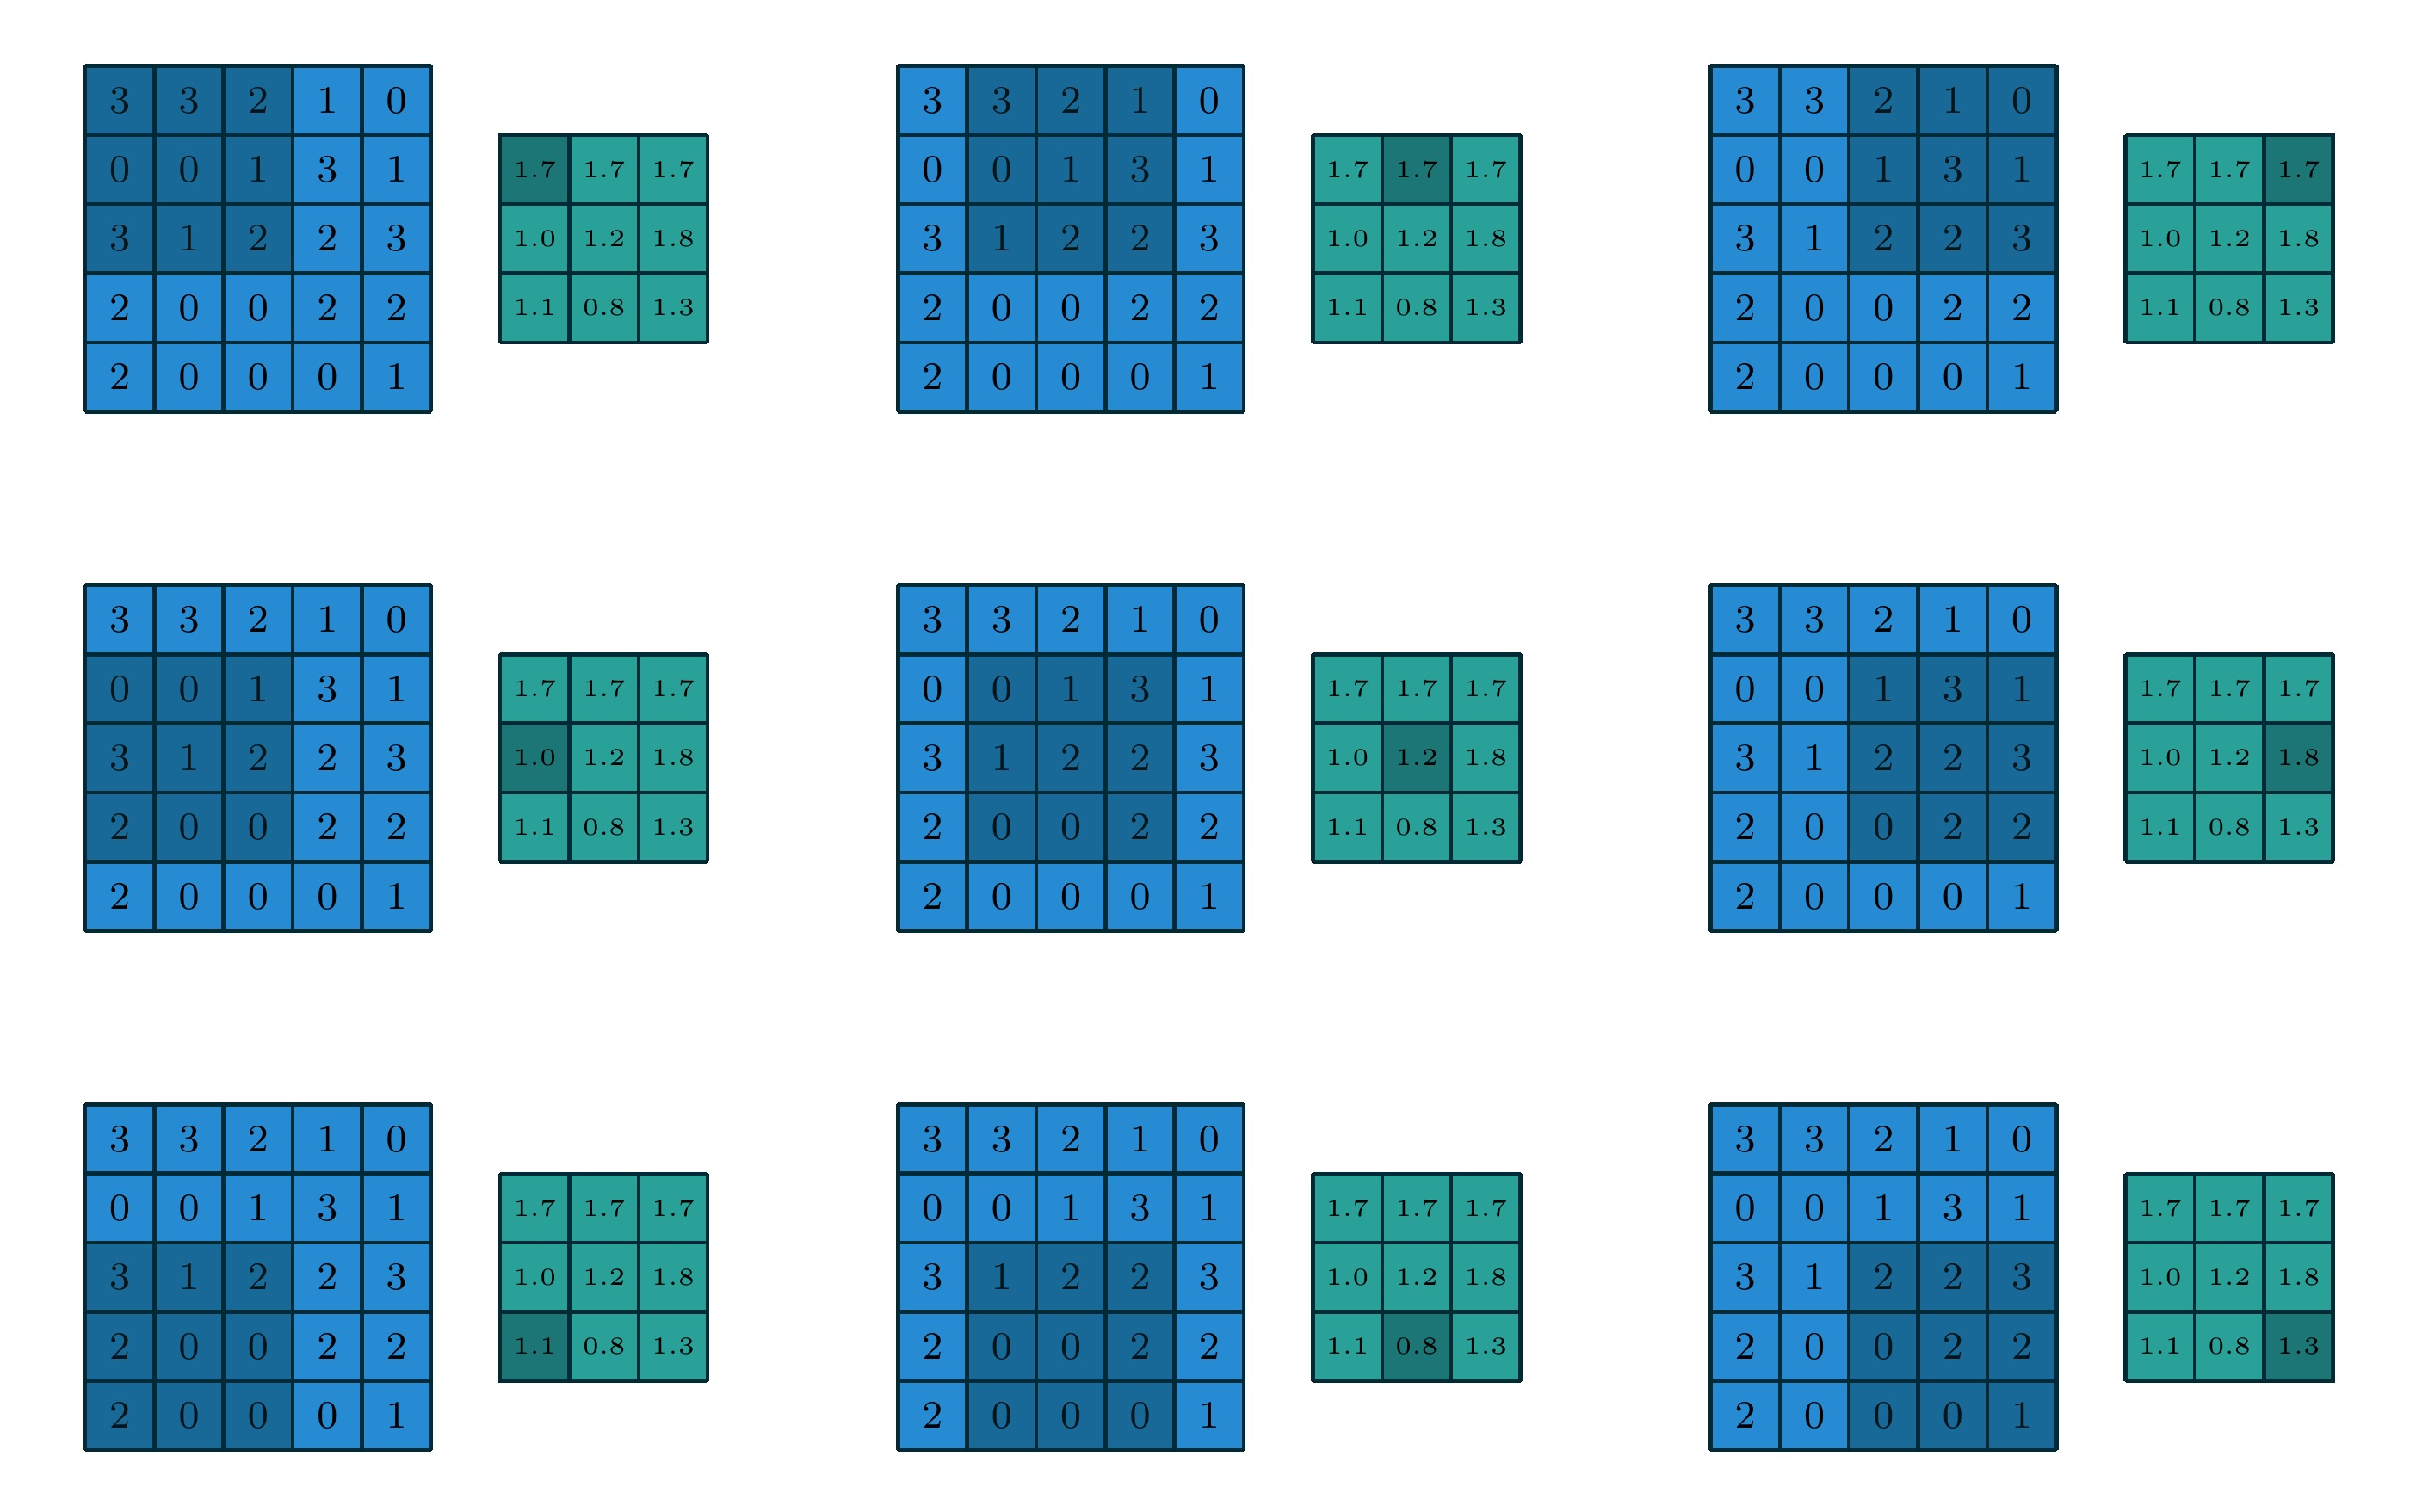
\includegraphics[width =0.9\textwidth]{images/convolucion/ima15.jpg}
    \caption{\gls{Pooling} por promedio}
    \label{fig:poolMax}
\end{figure}
\begin{figure}[H]
    \centering
    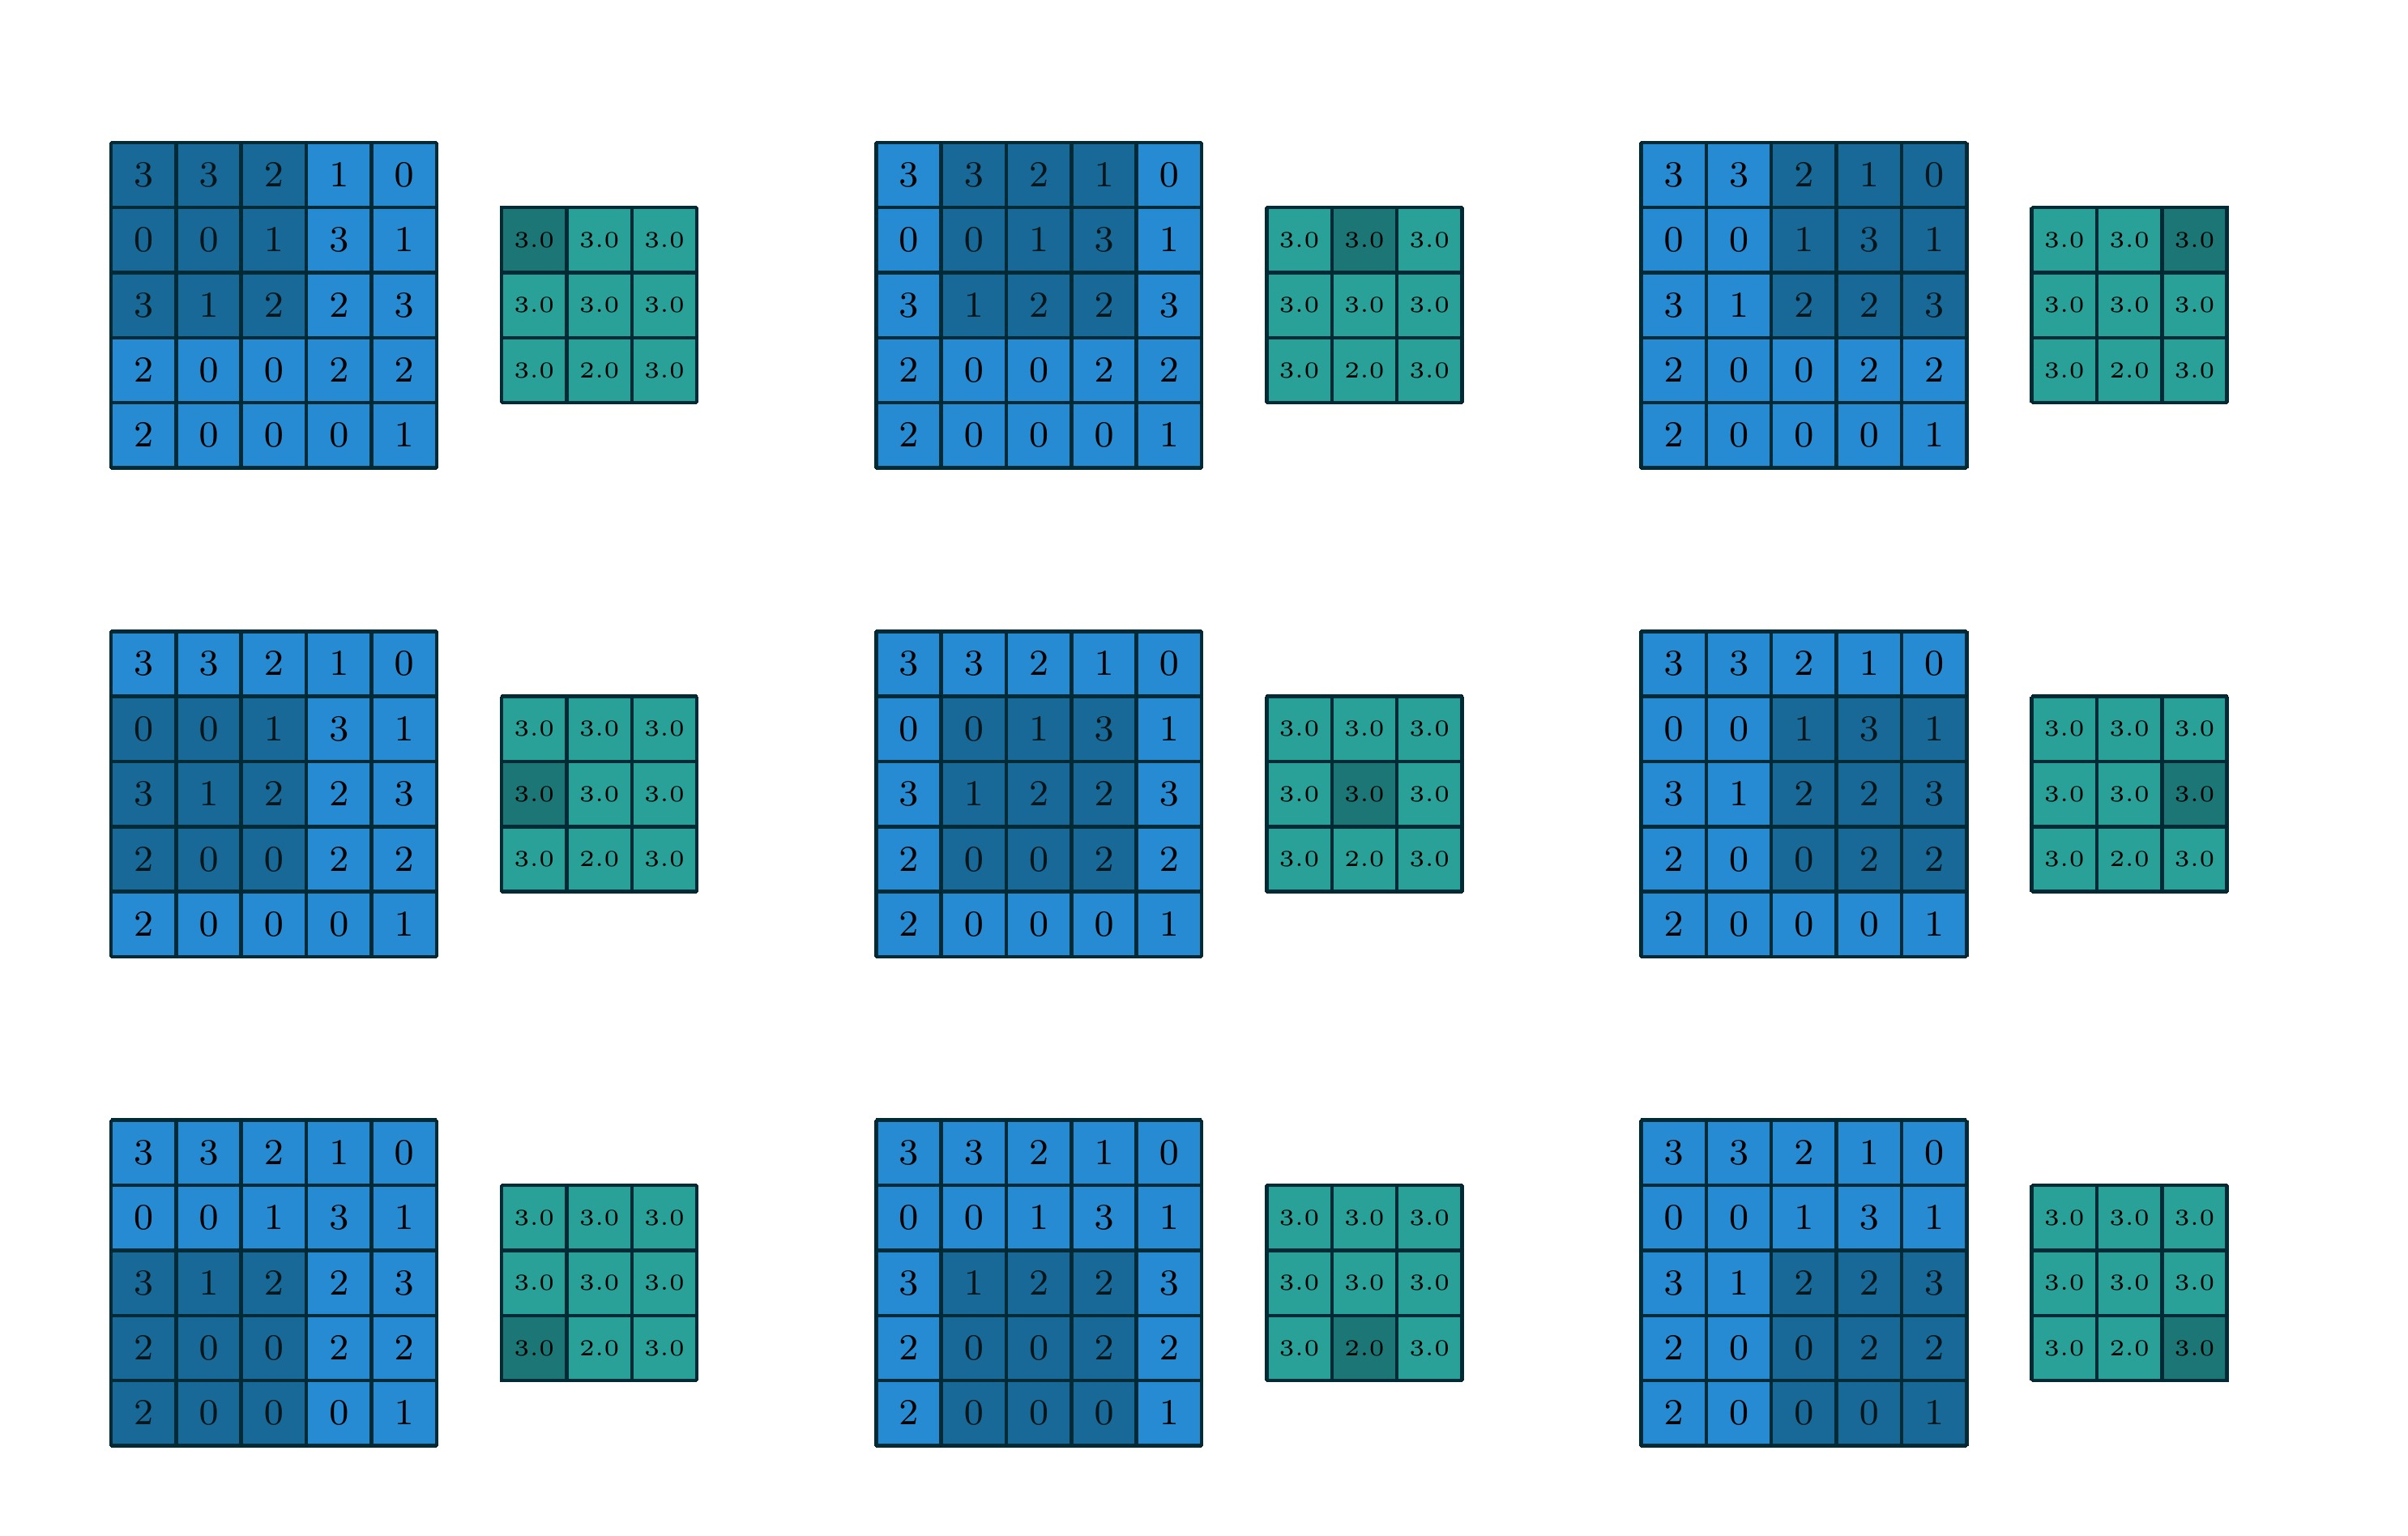
\includegraphics[width =0.9\textwidth]{images/convolucion/ima16.jpg}
    \caption{\gls{Pooling} por valor máximo}
    \label{fig:poolAverage}
\end{figure}

El valor de la salida de esta operaciones cuya entrada es de tamaño (N, C, H, W), salida = N, C, $H_{out}$, $W_{out}$ y de tamaño de \gls{kernel} $kH$, $kW$ puede ser descrito por la siguiente fórmula
\begin{equation}
\begin{split}
    out(N_i,C_J,h,w)=  &\max_{m=0 ,..., kH-1}\max_{n=0 ,...,kW-1}    \\
    &input(N_i,C_j,\gls{Stride}[0]\times h+m,\gls{Stride}[1]\times w+n)
\end{split}
\end{equation}

El \gls{Pooling} puede presentar los siguientes parámetros 
\begin{itemize}
    \item  \textbf{Tamaño de \gls{kernel}:} El tamaño de la ventana

    \item    \textbf{Stride:} El desplazamiento de la ventana, lo normal es que este sea del tamaño del \gls{kernel}.

    \item    \textbf{Padding:} Valores de zero agregado en los bordes.

    \item    \textbf{Dilation:} Controla la separación entre los cuadros de la ventana, se aprecia en la \figurename~\ref{fig:dilatation}
    
\end{itemize}{}

        


De lo anterior se obtienen las siguientes dimensiones:
        Input: (N, C, $H_{in}$, $W_{in}$)
        
        Output: (N, C, $H_{out}$, $W_{out}$) donde
        
        
        \begin{equation}
         H_{out}= \frac{H_{in}+2\times padding[0]-dilation[0]\times (\gls{kernel}\_size[0]-1)-1}{stride[0]} +1  
        \end{equation}
        \begin{equation}
         W_{out}= \frac{W_{in}+2\times padding[1]-dilation[1]\times (\gls{kernel}\_size[1]-1)-1}{stride[1]} +1  
        \end{equation}
        



\subsubsection{Convolución Transpuesta}
\label{sub:convolucionTranspuesta}
La necesidad de la convolución transpuesta generalmente llega a partir del deseo de usar una transformación en la dirección opuesta de la convolución normal, por ejemplo si deseamos obtener el tamaño de la entrada mientras se mantiene un patrón de conectividad. Esta operación es usada en lo decodificadores y el upsampling de varias redes neuronales.

Como por ejemplo en la \figurename~\ref{fig:convolucionNormal}. Si la entrada y la salida fueran desenrollados en vectores de izquierda a derecha, de arriba a abajo, la convolución podría ser representada como una matriz dispersa donde los elementos que no sean zeros son los elemento w, i, j del \gls{kernel} donde i y j es la fila y la columna respectivamente

\setcounter{MaxMatrixCols}{20}
\begin{figure}[H]

\begin{adjustbox}{max width=\textwidth}
\begin{bmatrix}
W_{0,0} & W_{0,1} & W_{0,2} & 0 & W_{1,0} & W_{1,1} & W_{1,2}& 0 & W_{2,0} & W_{2,1} & W_{2,2} & 0 & 0 & 0 &  0 & 0 \\
0 & W_{0,0} & W_{0,1} & W_{0,2} & 0 & W_{1,0} & W_{1,1} & W_{1,2}& 0 &W_{2,0} & W_{2,1} & W_{2,2}& 0 & 0 & 0&  0 \\
0 & 0 & 0&  0 & W_{0,0} & W_{0,1} & W_{0,2} & 0 & W_{1,0} & W_{1,1} & W_{1,2}& 0 &W_{2,0} & W_{2,1} & W_{2,2}&  0 \\
0 & 0 & 0 &  0 & 0 & W_{0,0} & W_{0,1} & W_{0,2} & 0 & W_{1,0} & W_{1,1} & W_{1,2}& 0 &W_{2,0} & W_{2,1} & W_{2,2}
\end{bmatrix}
\end{adjustbox}

\caption{Matriz C que representa la operación de convolución de la \figurename~\ref{fig:convolucionNormal}}
\label{fig:convolucionComoMatriz}
\end{figure}{}
Esta operación lineal toma la entrada de la matriz aplanada como un vector de 16 dimensiones y produce un vector de 4 dimensiones que es después es reconstruido a una matriz de 2 por 2.  Usando esta representación, el paso contrario puede ser obtenido fácilmente al transponer la matriz $C$, en otras palabras, el error es retropropagado por multiplicar la perdida con $C^T$. Esta operación toma un arreglo de dimensión 4 como entrada y produce y arreglo de 16 dimensiones como salida. Es notable que el \gls{kernel} w define ambas matrices $C$ y $C^T$

La Convolución Transpuesta llamada(también fractionally strided o deconvolución\footnote{El termino deconvolución aveces es usado en la literatura, pero no esta del todo bien utilizado debido a que en matemática la deconvolución es la operación inversa de la convolución}) funciona invirtiendo los pasos de forward y backward de una convolución. Es notorio que el \gls{kernel} define una convolución directa o una convolución transpuesta pero el determinar si es una u otra depende de como se computa el forward y el backward. Por ejemplo, aunque el \gls{kernel} w define una convolución cuyos pasos de forward and backward son computados por la multiplicación de $C^T$ y $(C^T)^T=C$ respectivamente\footnote{La convolución transpuesta puede ser pensada como la gradiente de alguna convolución con respecto a la entrada, que es de hecho como las convoluciones transpuestas son implementadas en practica}

\begin{figure}[H]
    \centering
    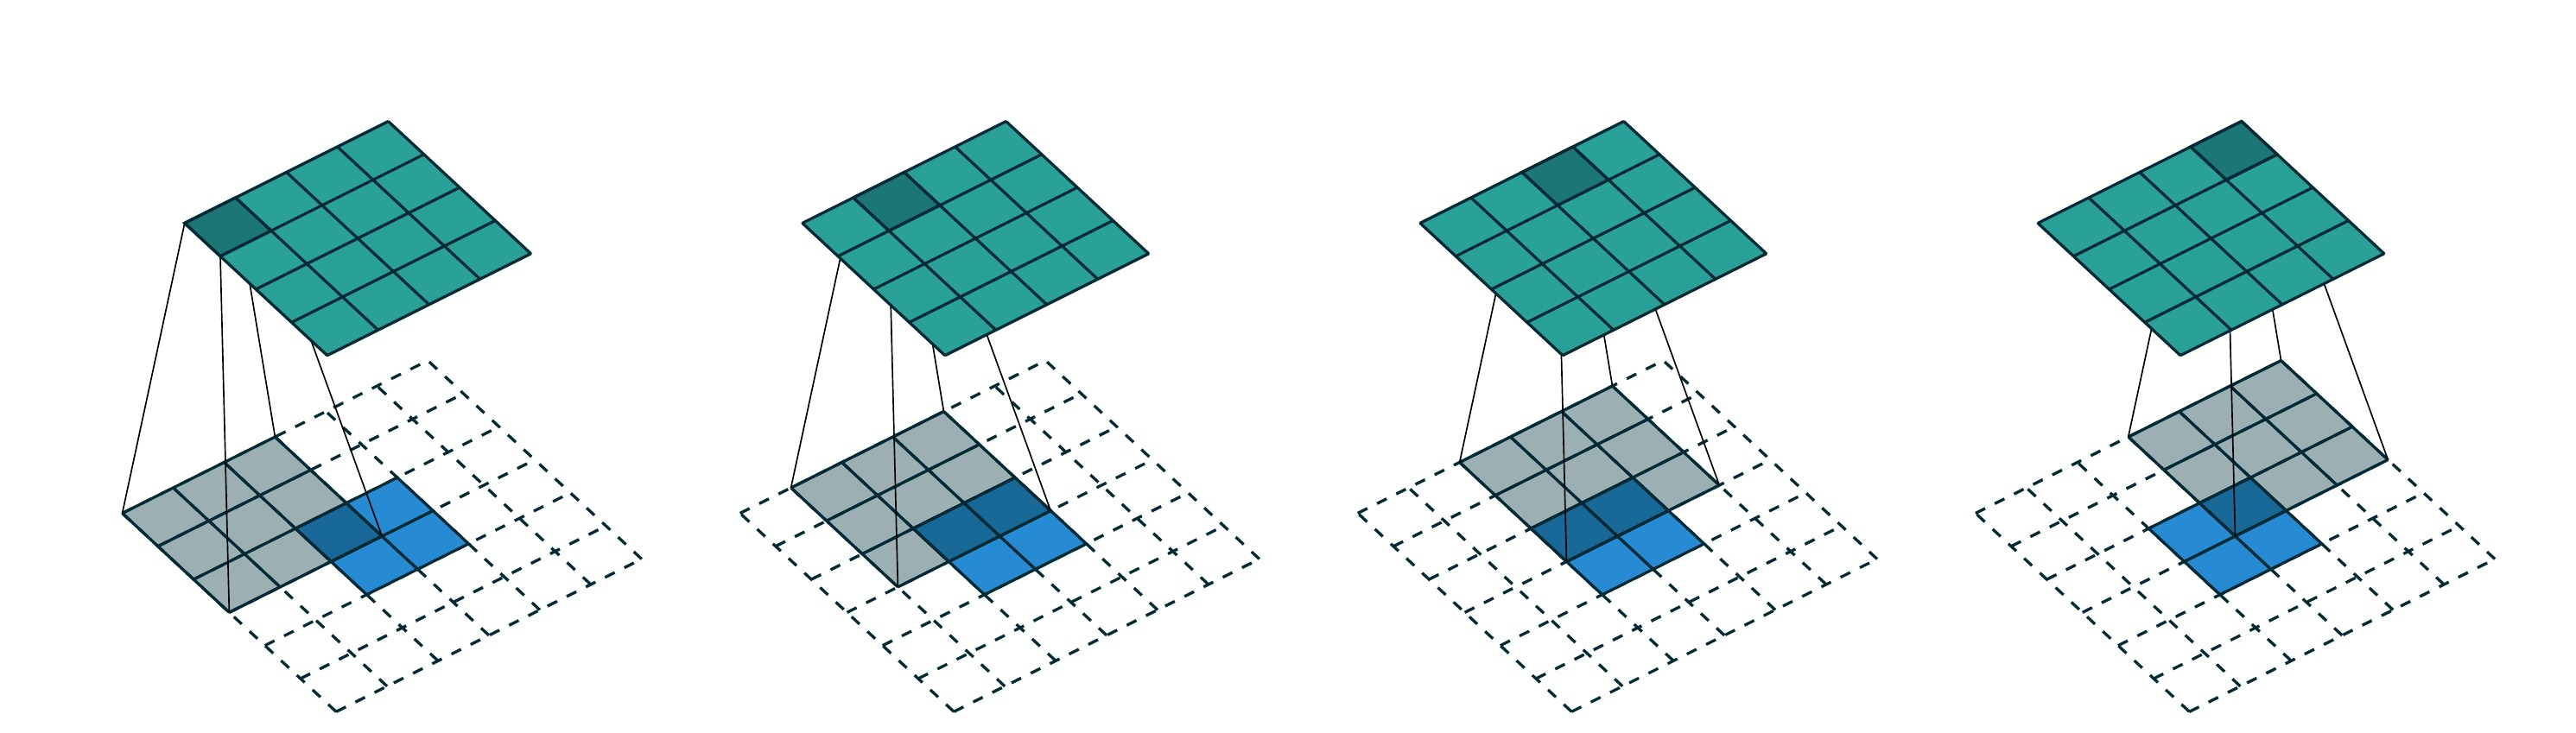
\includegraphics[width =0.9\textwidth]{images/convolucion/ima41.jpg}
    \caption{Muestra de convolución transpuesta}
    \label{fig:my_label}
\end{figure}
Los parámetros manejados para la convolución transpuesta son 
\begin{itemize}
    \item   \textbf{Stride} controla el desplazamiento del \gls{kernel}.

    \item \textbf{Padding} controla la cantidad de zeros en los bordes.

    \item \textbf{Output\_padding} Controla la cantidad de zeros agregados en la salida.

    \item \textbf{Dilation} controla el espacio entre los elementos del \gls{kernel}\ref{fig:dilatation}.

    \item \textbf{Groups} controla las conexiones entre la entrada y la salida, se aprecia mejor en la \figurename~\ref{fig:convolucionGrupos}
    \begin{itemize}
        \item  Con groups=1, todos los elementos de la entrada se convolución en los de la salida.

        \item    Con groups=2, la operación se vuelve equivalente a tener 2 capas, cada uno viendo solo la mitad de los canales de entrada .

     

    \end{itemize}
            
\end{itemize}
   
De lo anterior mencionado se puede calcular lo siguiente.
        Input: (N, $C_{in}$, $H_{in}$, $W_{in}$)
        Output: (N, $C_{out}$, $H_{out}$, $W_{out}$) donde

        
        \begin{equation}
            H_{out} = \frac{H{in}+2\times padding[0]-dilation[0]\times (\gls{kernel}\_size[0]-1)-1}{stride[0]} +1
        \end{equation}
         
        \begin{equation}
            W_{out} = \frac{W{in}+2\times padding[1]-dilation[1]  \times (\gls{kernel}\_size[1]-1)-1}{stride[1]} +1
        \end{equation}
        
    Siendo N el tamaño de \gls{Batch} , $C_{in}$ y $C_{out}$ la cantidad de canales de entrada y salida respectivamente, $H_{in}$ y $H_{out}$ la altura de la entrada y salida respectivamente , $W_{in}$ y $W_{out}$ el ancho de la entrada y salida respectivamente.



    
\subsubsection{DropOut}

Aleatoriamente convierte a zero un canal\footnote{ Un canal es un \gls{Feature Map} de 2 dimensiones}. Cada canal sera convertido a zero independientemente en cada llamada a forward con una probabilidad $p$, es usual usar la distribución de Bernolli. 

Como se describe en el artículo \cite{Tompson2014}, si los pixeles adyacentes dentro de los mapas de características están fuertemente correlacionados (como suele ocurrir en las primeras capas convolucionales), entonces el Dropout no regularizará las activaciones y, de lo contrario, solo resultará en una disminución efectiva de la tasa de aprendizaje.


\subsubsection{Normalización por batches}
 Según \cite{Ioffe2015} el entrenamiento en las redes neuronales profundas se complica por el hecho de que la distribución de las entradas de cada capa cambia durante el entrenamiento, a medida que cambian los parámetros de las capas anteriores. Esto ralentiza el entrenamiento al requerir tasas de aprendizaje más bajas y una cuidadosa inicialización de parámetros, y hace que sea extremadamente difícil entrenar Modelos con saturación no lineales. Nos referimos a este fenómeno como cambio de covariables internas y resolvemos el problema al normalizar las entradas de capa. El método propuesto por \cite{Ioffe2015} se basa en hacer de la normalización una parte de la arquitectura del modelo y realizar la normalización para cada mini batch de entrenamiento. La normalización por lotes nos permite utilizar índices de aprendizaje mucho más altos y ser menos cuidadosos con la inicialización. También actúa como regulador, en algunos casos eliminando la necesidad de abandono. 
 \begin{equation}
     y = \frac{x-E[x]}{\sqrt{var[x]+\epsilon}}
 \end{equation}

Donde:
\begin{itemize}
    \item \textbf{y} es el valor esperado. 
    \item \textbf{x} es el mini \gls{Batch}.
    \item \textbf{E[x]} es el promedio.
    \item \textbf{var[x]} es la varianza.
\end{itemize}{}


\subsection{Frameworks de Desarrollo}
    \paragraph{Tensorflow:} Es una biblioteca para el aprendizaje automático de código abierto para investigación y producción utilizada para el cálculo numérico mediante diagramas de flujos de datos. Los nodos de los diagramas representan operaciones matemáticas y las aristas las matrices de datos multidimensionales (tensores) comunicadas entre ellas. Se necesita una API para desplegar el sistema informático de una o varias CPU o GPU. TensorFlow fue desarrollado por el ``Google Brain Team'' que formaban parte de la organización de investigación de aprendizaje automático de Google~\cite{Brain2015}.
   
    \paragraph{Keras:}Keras es una \gls{API} de redes neuronales de alto nivel para la construcción y entrenamiento de modelos de aprendizaje profundo, implementada en Python y capaz de ejecutarse sobre TensorFlow, CNTK o Theano. Fue desarrollado con el objetivo de permitir una experimentación rápida en investigación avanzada y producción~\cite{Brain2015}.
    Según~\cite{Chollet2015} Keras permite: 
    \begin{itemize}
        \item Realizar prototipos rápidamente (facilidad de uso, modularidad y extensibilidad).
        \item El uso de \gls{CNN},  \gls{RNN} y sus variaciones.
        \item El funcionamiento sobre \gls{CPU} y \gls{GPU}.
    \end{itemize}
    
    \paragraph{Pytorch:} Es una biblioteca tensor optimizada para la manipulación de matrices de datos empleadas en aprendizaje profundo utilizando \gls{GPU} y \gls{CPU}, esta basado en Torch y desarrollado por el grupo de inteligencia artificial de Facebook~\cite{Paszke2016}.
    Pytorch se caracteriza por:
    \begin{itemize}
        \item Cálculo tensorial acelerado.
        \item Entrenamiento distribuido.
        \item Integración profunda en Python.
        \item Soporte nativo de ONNX (Open Neural Network Exchange).
    \end{itemize}
    
    \paragraph{Caffe:} Es un framework de aprendizaje profundo desarrollado teniendo en cuenta la expresión, la velocidad y la modularidad. Fue implementado por ``Berkeley AI Research ( BAIR)'' y por colaboradores de la comunidad. Yangqing Jia creó el proyecto durante su doctorado en UC Berkeley. Caffe se lanza bajo la licencia BSD 2-Clause~\cite{Jia2015}.
   
    \paragraph{Theano:} Theano es una biblioteca de Python que permite definir, optimizar y evaluar expresiones matemáticas con matrices multidimensionales de manera eficiente~\cite{Theano2011} Características de Theano:
    \begin{itemize}
        \item Integración con NumPy\footnote{NumPy es una extensión de Python, que le agrega mayor soporte para vectores y matrices, constituyendo una biblioteca de funciones matemáticas de alto nivel para operar con esos vectores o matrices}.
        \item Uso transparente de una \gls{GPU}.
        \item Optimizado en velocidad y estabilidad.
        \item Genera dinámicamente codigo C.
        \item Disponibilidad de pruebas.
    \end{itemize}



\section{Redes neuronales en Segmentación semántica}
Como se menciona en el artículo de~\cite{long2015fully} el uso de las redes neuronales para la clasificación de imágenes cobro bastante importancia desde que el trabajo de~\cite{krizhevsky2012imagenet} en 2012 gano el concurso Imagenet que consistía en etiquetar imágenes, a partir de eso distintos trabajos comenzaron a hacer el uso de las redes neuronales convolucionales para etiquetado de imágenes y para la detección de objetos.
El próximo paso fue la inferencia de cada pixel, los primeros intentos para la segmentación semántica~\cite{ning2005toward ,   ciresan2012deep , farabet2013learning} realizaban una clasificación para cada uno de los pixeles tomando en cuenta una ventana, es decir se utilizaba una red neuronal para cada pixel. Usar una red neuronal para clasificar cada uno de los pixeles es bastante costoso e ineficiente debido a que parte de las redes que pueden ser utilizados, en el paper de~\cite{long2015fully} indica que la red de propuesta en \cite{krizhevsky2012imagenet}  realiza la tarea de clasificación de una imagen de 224x224 en 1.2 ms mientras que la arquitectura propuesta  puede generar una grilla de 10x10 de una imagen de 500x500 en 22 ms logrando asi una velocidad 5 veces mayor al enfoque primitivo de clasificar cada pixel.

\subsection{Fully Convolutional Network}
La \gls{FCN}(Fully Convolutional Network) original aprende un mapeo de pixeles a pixeles\cite{long2015fully}. El canal de la red \gls{FCN} es una extensión de la \gls{CNN} clásica. La idea principal es hacer que la \gls{CNN} clásica tome como entrada imágenes de tamaño arbitrario. La restricción de las \gls{CNN} para aceptar y producir etiquetas solo para entradas de tamaño específico proviene de las capas totalmente conectadas que son fijas. Contrariamente a ellos, las \gls{FCN} solo tienen capas convolucionales y de agrupación que les dan la capacidad de hacer predicciones sobre entradas de tamaño arbitrario. 


\begin{figure}[H]
    \centering
    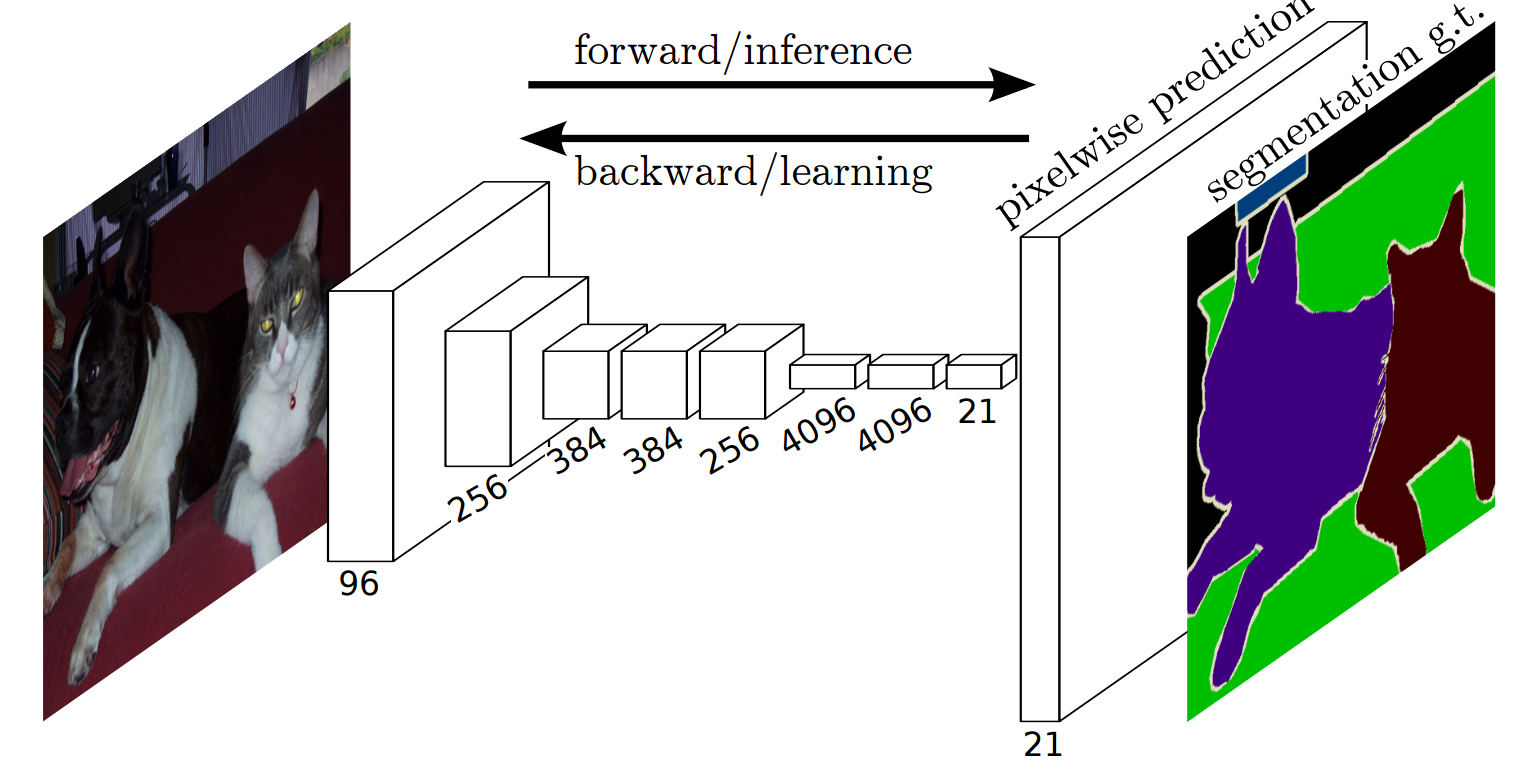
\includegraphics[width = 0.8\textwidth]{images/cat_segmentation.png}
    \caption{Arquitectura de \gls{FCN} obtenida de \cite{long2015fully}}
    \label{fig:my_label}
\end{figure}
La característica de las \gls{FCN} es que estas poseen 2 partes principalmente.
\begin{itemize}
        \item \textbf{Codificador} Este modulo gradualmente reduce el mapa de características y captura la mayor cantidad de información semántico.
        \item \textbf{Decodificador} : Este modulo gradualmente recupera la información espacial 
    \end{itemize}{}
    
    

\section{Técnicas tradicionales del Análisis forestal}
\subsection{Índices de vegetación }
Según la hoja de apuntes de~\cite{munoz2017apuntes} se pueden clasificar los índices en 2 :
\subsubsection{Índices Basados en la Pendiente}
Los índices basados en la pendiente usan el cociente de la reflectancia de una banda con otra, usualmente el rojo y el \gls{IR} cercano, debido al alto contraste o diferencia en la reflectancia, que presenta la clorofila1en ambas bandas. El término ‘basado en la pendiente’ se refiere a que, al analizar los valores resultantes del índice de vegetación, se compararán esencialmente las pendientes de las líneas que pasan a través del origen y de los pixeles representados en un gráfico, con la reflectancia de una banda en el eje de las X y la reflectancia de la otra en el eje Y.


\begin{figure}[H]
    \centering
    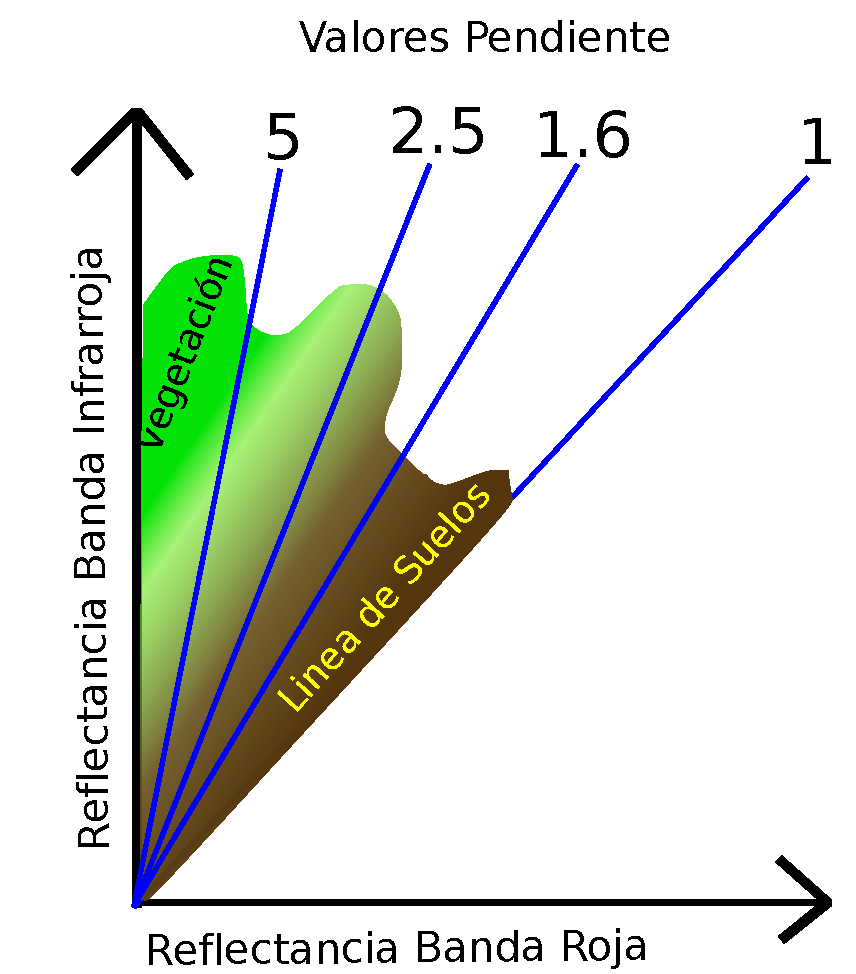
\includegraphics[width=0.4\textwidth]{images/indiceVegetacion.pdf}
    \caption{Gráfica de simulación de índices de vegetación adaptada de~\cite{munoz2017apuntes} }
    \label{fig:indicesBasadosEnLaPendiente}
\end{figure}
\begin{table}[H]
    \centering
    \begin{tabular}{|M{0.10\textwidth}|M{0.35\textwidth}|
   M{0.4\textwidth}|M{0.10\textwidth}| }\rowcolor[HTML]{EFEFEF} 
        \hline Nombre del Índice & Fórmula & Características & Autor y año \\ \hline
  NDVI Diferencia normalizada &$ \scriptsize{NDVI = \frac{NIR-RED}{NIR+RED}} $ & \scriptsize {Minimiza efectos topográficos y produce escala lineal de medición. La escala va de –1 a 1 con el valor cero representando el valor aproximado donde empieza la ausencia de vegetación. Los valores negativos representan superficies sin vegetación.La normalización que realiza, reduce el efecto de la degradación de calibración del sensor y la influencia de los efectos atmosféricos. Gran sencillez matemática.} & Rouse et al.\cite{rouse1973monitoring} \\\hline 
  TVI Transformado& $\scriptsize{NDVI =\sqrt{ \frac{NIR-RED}{NIR+RED}+0.5 }} $ & \scriptsize{El 0,5 evita valores negativos. La raíz cuadrada, intenta corregir los valores que se aproximan a una distribución de Poissone introduce una distribución normal. No elimina todos los valores negativos.} &Rouse et al. \cite{rouse1973monitoring}\\ \hline
 TTVI Transformadade Thiam & $\scriptsize{TTVI = \sqrt{ABS(NDVI + 0.50)}}$ & \scriptsize{El 0.5 corrige la sobre estimación del verde del TVI} &Richardson et al. \cite{richardson1977distinguishing} \\ \hline
 RVI2 Cociente simple & $RVI =\frac{NIR}{RED} $ & \scriptsize{Poco sensible a las condiciones de iluminación, pero mucho a las propiedades ópticas de la tierra.} &Pearson y Miller \cite{pearson1972remote} \\ \hline 
 NRVI3 Cociente simple normalizado&$NRVI = \frac{RVI –1}{RVI + 1}$& \scriptsize{El resultado del NRVI es normalizado. Es similar al NDVI, reduce los efectos de la topografía, la iluminación y los efectos atmosféricos, además de crear una distribución  normal  estadísticamente deseable.}& Perry y Lautenschlager \cite{perry1984functional} \\ \hline 
 NDWI Diferencial de agua normalizado &$NDWI = \frac{NIR -SWIR}{NIR+SWIR} $& \scriptsize{Este índice se utiliza para medir la cantidad de agua que posee la vegetación o el nivel de saturación de humedad que posee el suelo. Los valores que se obtienen oscilan entre -1 y 1, para las zonas con menos humedad}. & Clevers \cite{clevers1988derivation}\\ \hline 
    \end{tabular}
    \caption{Tabla de Índices de Vegetación}
    \label{tab:my_label}
\end{table}

\subsubsection{Índices Basados en la Distancia}
Los valores de reflectancia registrados por el sensor, para cada pixel, constituyen una reflectancia promedio de todos los tipos de coberturas que están dentro desee pixel. Cuando en  zonas áridas y semi áridas la vegetación es dispersa, la reflectancia recibida pertenece tanto a vegetación como suelo. Estos índices, que tratan de separar la información entre la vegetación y el suelo, se basan en el uso de una línea del suelo y las distancias desde ella


\section{Métodos de validación de resultados}
\subsection{Matriz de confusión}
Es una forma gráfica de análisis del desempeño de los algoritmos de clasificación, usualmente se usa con dos clases para etiquetarlos como falsos o verdaderos para definir la predicción y positivos o negativos para definir la clase real de pertenencia, en la \figurename~\ref{figure:confusionmatrix} se puede apreciar una matriz de confusión para un problema de más de dos clases, para este tipo de matrices se considera la diagonal principal en tonalidades rojo como True Positives, por ejemplo para la clase cero se tiene 34 instancias de las cuales 34 han sido clasificadas correctamente, sin embargo para la clase tres se tiene un total de 41 instancias de las cuales sólo 36 fueron clasificadas correctamente y 5 en tonalidades de amarillo fueron clasificadas como otras clases, \begin{figure}[h]
	\centering
	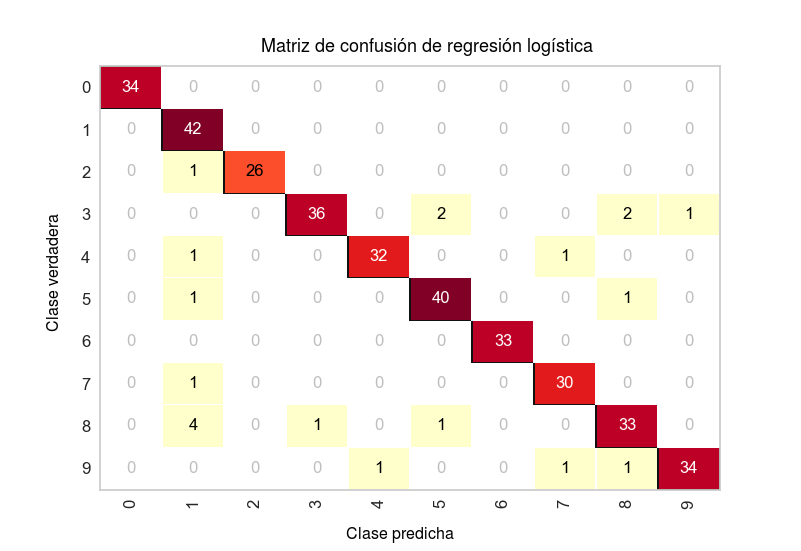
\includegraphics[width=\textwidth]{images/02theory/confusionMatrixEspa.png}
	\caption{Matriz de confusión con más de dos clases, se consideran relevantes los valores de la diagonal principal.}
	\label{figure:confusionmatrix}
\end{figure}


\subsection{Recall y Precisión}
La existencia de muchas instancias negativas es un fenómeno común en muchos sub-campos de la minería de datos y el aprendizaje máquina, por ejemplo muchas de las páginas web son irrelevantes para muchas peticiones. El Accuracy no es una medida de evaluación sensible a la existencia de muchas instancias negativas. Una buena solución es el ignorar los casos que son verdaderos negativos y usar métricas como Recall y Precisión~\cite{Flach2015}
La Precisión esta definida como:
\begin{equation}
 \text{Precision}  = \frac{TP}{TP+FP}
\end{equation}
Donde:
\begin{itemize}
\item \textbf{TP: True Positive} Cantidad de predicciones positivas hechas correctamente.
\item \textbf{FP: False Positive} Cantidad de predicciones positivas hechas incorrectamente.
\end{itemize}

Luego el Recall esta definido como: 

\begin{equation}
 \text{Recall}  = \frac{TP}{TP+FN}
\end{equation}


Donde:
\begin{itemize}
\item \textbf{TP: True Positive} Cantidad de predicciones positivas hechas correctamente.
\item \textbf{FN: False Negative} Cantidad de predicciones negativas hechas incorrectamente.
\end{itemize}
Una forma adicional que mide la relación de desempeño entre el precision y recall es denominada \textbf{F-Measure} definida como:
\begin{equation}
\text{F-Measure}= \frac{2*P*R}{P+R}    
\end{equation}

donde:
P es la precision y R la recall para cierto conjunto de datos.




\section{Segmentación Semántica}
\label{section:metricsevaluation}
\subsection{Métricas para validación de segmentación semántica}
Para que los resultados de segmentación sean buenos se deben usar métricas bien establecidas que permitan validar la utilidad del sistema, en el estado del arte tenemos:
\begin{itemize}
	\item \textbf{Tiempo de ejecución:} Debido al costo computacional de las técnicas utilizadas, es importante conocer el tiempo de entrenamiento de cada una de ellas, es necesario conocer tiempos de cómputo que dependen de hardware específico, brindar tiempos exactos para ciertas configuraciones que permitan tomar decisiones de costos y reproducibilidad de experimentos.
	\item \textbf{Espacios de memoria:} Puede ser un elemento limitante en caso de los modelos que consuman bastante memoria, mantener un reporte de la cantidad de memoria a lo largo de la ejecución del programa se considera necesario para reproducción de experimentos.
	\item \textbf{Accuracy:}  Consiste de métricas que miden la relación del etiquetado por pixel con su objetivo, usualmente variaciones en las precisiones por pixel.
     \begin{itemize}
			\item \textbf{Pixel Accuracy (PA):} Calcula la relación entre el total de pixeles correctamente clasificados y el total de pixeles, definido como: 
			\begin{equation}
			    \text{PA} = \frac{\sum^k_{i=0}p_{ii}}{\sum_{i=0}^{k}\sum_{j=0}^{k} p_{ij}}
			    \end{equation}
			\item \textbf{Mean Pixel Accuraccy (MPA):} Similar al PA descrito arriba con la diferencia de calcular la relación de pixeles correctamente clasificados por clase y luego promediar con el total de clases, se define así:
				\begin{equation}
				\text{MPA} = \frac{1}{k+1}\sum_{i=0}^k\frac{p_{ii}}{\sum_{j=0}^kp_{ij}}
				\end{equation}
			\item \textbf{Mean Intersection over Union (MIoU):} este es el método estándar de evaluación, calcula la relación entre la intersección y la unión de dos conjuntos, en segmentación esto es la relación entre nuestro \textbf{ground truth} y nuestra predicción, se define así: 
			\begin{equation}
			\text{MIoU}= \frac{1}{k+1}\sum_{i=0}^k\frac{p_{ii}}{\sum_{j=0}^k p_{ij}+\sum_{j=0}^{k}p_{ji}-p_{ii}}
			\end{equation}
			\item \textbf{Frecuency Weighted Intersection over Union (FWIoU):} mejora la métrica anterior ponderando la importancia de cada clase con su frecuencia de aparición, definida como:
				\begin{equation}
				    				\text{FWIoU}= \frac{1}{\sum_{i=0}^k \sum_{j=0}^kp_{ij}}\sum_{i=0}^k\frac{\sum_{j=0}^kp_{ij}p_{ii}}{\sum_{j=0}^kp_{ij}+\sum_{j=0}^{k}p_{ji}-p_{ii}}
				    				\end{equation}
		  \end{itemize}
\end{itemize}
Según~\cite{GarciaGarcia2017} \textbf{MIou} es la métrica más usada debido a su simplicidad y representatividad.
\paragraph{Coeficiente de similaridad de Jaccard:} Los índices de similitud son utilizados para el estudio de coexistencia de especies o similitud de sitios de muestreo. Una matriz de coeficientes de similitud, de especies o ubicaciones puede analizarse de dos maneras: por ordenación, es decir, al intentar organizar las ubicaciones o especies dentro de una secuencia teórica continua, o por clasificación, donde se colocan las ubicaciones o especies en grupos discontinuos.
Una manera general como se expresa Jaccard en~\cite{Real1996} es:
\begin{equation}
    J = \frac{C}{A+B-C}
\end{equation}
donde:
\begin{itemize}
    \item A es el número de atributos presentes en un conjunto a.
    \item B es el número de atributos presentes en un conjunto b.
    \item C es el número de atributos presentes en ambos conjuntos a y b.
\end{itemize}
Al coeficiente de Jaccard se le denomina también Intersection over Union, pero para este reporte consideramos Jaccard o \gls{iou}.
\section{Estado del Arte}

En~\cite{Gomez2015} se muestra el desarrollo de metodología para la detección de cambios en series temporales de imágenes Landsat, el autor rellena los datos no útiles (causados por nubes u otros) mediante una interpolación, también el autor plantea una técnica para tratar de predecir el estado actual del bosque basado en la serie temporal, sin embargo demostró que sus resultados de análisis dependen mucho de una data consistente.


El trabajo de~\cite{Vogelmann2012} es un estudio de cambios en varios bosques de Estados Unidos, para esto usaron series temporales de imágenes Landsat, siendo el principal medio de análisis una regresión lineal sobre el Índice Normalizado de Vegetación (NDVI por sus siglas en ingles). El estudio demostró que existen bastantes lugares en los cuales la deforestación va en aumento pero también lugares en los que se esta reforestando.

En~\cite{Saxena2018} menciona que existen distintos algoritmos para la detección de cambios en imágenes satelitales, no obstante el autor menciona que estos algoritmos fueron diseñados para su conjunto de datos, entonces el autor propone usar un conglomerado de algoritmos decidiendo cual usar basado en la distancia de Hausdorff. 


En~\cite{Brooks2017} se muestra las deficiencias de los algoritmos de detección de deforestación causada por factores no tan comunes como son: sequía, enfermedad, actividad de insectos y raleo de cosechas, se propone un algoritmo especializado en detectar los cambios que provienen de dichos factores, su algoritmo esta basado en estadística.


Al igual que el trabajo de~\cite{Saxena2018}, el trabajo~\cite{Healey2018} utiliza la combinación de varios algoritmos, el trabajo se realizó con 8 algoritmos funcionados mediante reglas de fusión basadas en Random Forest, se demuestra la validez de su enfoque probando su algoritmo en imágenes satelitales de varios satélites.

En~\cite{Dutrieux2016} se trata de reconstruir el historial de cambios en base a una serie temporal de imágenes satelitales, para hacer esto utiliza el BFAST (framework Breaks For Additive Season and Trend) que esta especializado en predecir este tipo de actividades, el algoritmo que usaron fue: NDMI (Normalized Difference Moisture Index). En el trabajo se utilizaron todas las imágenes Landsat 7 disponibles de la zona de estudio hasta 5 meses antes de la fecha de publicación. 

% qwerty123
En~\cite{Schroeder2014} muestra como el uso de 2 tipos de imágenes (Landsat y fotografías aéreas) obtienen un resultado con mejor claridad, la primera parte de la metodología incluye una detección de cambios utilizando series temporales Landsat, como consecuencia el uso de la fotografía aérea puede ser más focalizado logrando así reducir costos.

%Se han desarrollado distintos trabajos relacionados a la detección de cambios de suelos Se puede mencionar algunos de los trabajos como son los de :~\cite{Zhu2017}\cite{Khan2016}~\cite{Khan2017}~\cite{Tan2016} que realizan una detección de cambios para un determinado dataset siendo el más común las escenas de LandSat.

%Además existen ciertos trabajos que utilizan redes neuronales para la detección de cambio de suelos como son los de Wang y Zhong\cite{Wang2014}\cite{Zhong2015}.Aunque ambos trabajen con diferente data ambos concuerdan con que trabajar por bloques de imágenes para el entrenamiento es la mejor opción.


%Las resolución subpixel es una herramienta útil para trabajar con imágenes de baja resolución espacial, en~\cite{Wang2014} se mostró que el uso de redes neuronales presenta mejores resultados a los trabajos realizados en resolución subpixel hasta antes de la fecha de publicación del articulo.



En~\cite{Zhong2015} se muestra que el uso de redes neuronales basadas en los sistemas nerviosos de mamíferos pequeños fue utilizado en la detección de cambios en imágenes satelitales, el trabajo combina una red ya estudiada con una característica ya calculada como es el momento normalizado de inercia, el autor indica que el uso combinado del momento de inercia y la red neuronal logra un mejor desempeño que el solo uso de la red neuronal.


En~\cite{SicongLiu2015} se muestra que los pixeles cambiados se pueden subcategorizar para obtener una mejor clasificación, el proceso propuesto por el autor comienza con una técnica basada en la resta de las imágenes, luego se clasifica los pixeles del resultado en 3 grupos, este proceso continua con cada grupo obteniendo, al final un árbol de clasificación en donde cada pixel pertenece a una hoja del árbol.



Otra técnica basada en clusters para la detección de cambios es la propuesta por~\cite{Leichtle2017}, la propuesta esta diseñada para la detección de nuevas edificaciones, el autor realiza un preprocesado basado en propiedades geométricas y análisis de componentes principales para concluir con una clasificación hecha con Kmeans.


Los algoritmos genéticos también pueden ser utilizados para el problema de detección de cambio, en el trabajo de~\cite{Kusetogullari2015} se muestra un método de detección que incluye el algoritmo genético de Particle Swarm Optimization, el autor hace énfasis en su función de fitness y su inicialización de su población para luego comparar su método con otros métodos no supervisados.

En~\cite{Vazquez-Jimenez2017} se trata de realizar la detección de cambios mediante patrones. Se uso como base el método de la transformación de la chi-cuadrada, aunque no se obtuvo resultados sobresalientes, estos fueron lo suficientemente buenos como para que el método se considere viable.

En el trabajo de~\cite{Maggiori2017} se muestra que el problema de etiquetar cada uno de los pixeles puede ser resuelto de distintas maneras. El trabajo muestra que el realizar una red neuronal para cada pixel es ineficiente, es por eso que el autor propone una \gls{FCN} para resolver el problema de una manera más óptima debido al hecho de que la información de pixeles continuos puede ser reutilizada.

